\documentclass{article}
\usepackage[utf8]{inputenc}
\usepackage[english]{babel}
\usepackage{xcolor}
\definecolor{light-gray}{gray}{0.95}
\usepackage{amsthm}
\newtheorem{theorem}{Theorem}
\newtheorem{proposition}{Proposition}
\newtheorem{definition}{Definition}
\usepackage{subfigure}
\usepackage{float}
\usepackage{lineno,hyperref}
\modulolinenumbers[5]
\usepackage{amssymb}
\usepackage{amsmath}
\usepackage{mdwtab}
\usepackage{url}
\usepackage{multirow}
\usepackage{float}
\usepackage{graphicx}
\graphicspath{{./figure/}}
\usepackage{fancyhdr}    % for headers and footers
\usepackage[colorlinks=true, linkcolor=black, urlcolor=blue, citecolor=black]{hyperref}
\hypersetup{
    pdfborder={0 0 0}
}
\usepackage{xcolor}
\usepackage{tikz}
\usepackage{lipsum}
\usepackage{listings}
\usepackage{newtxtext,newtxmath}
\usepackage{tipa} % for \textchi

\usepackage{mathtools}
\usepackage{setspace}
\usepackage{booktabs}
\usepackage{amssymb}
\usepackage{multirow}
\usepackage{array}
\usepackage{makecell}

\usepackage{fancyhdr} % For custom headers and footers
\usepackage{lipsum}   % For dummy text (optional)

\usepackage[margin=2.5cm]{geometry} % To control margins (if needed)

\usepackage{titlesec}
\usepackage{etoolbox}

\geometry{a4paper, margin=1in} % Adjust margins as necessary




\pagestyle{fancy}
\fancyhf{} % Clear all header and footer fields
\fancyhead[L]{Hamming code}
\fancyhead[R]{\makebox[\textwidth][r]{\textbf{\nouppercase{\leftmark}}}} % Right-alig

\fancyfoot[L]{\textbf{Department of ECE}} % Left side: Department name
\fancyfoot[C]{\textbf{Aug 2024 – Dec 2024}} % Center: Semester dates
\fancyfoot[R]{\textbf{Page \thepage}} % Right side: Page number
\renewcommand{\footrulewidth}{0.4pt}
\geometry{a4paper, margin=1in} % Adjust margins as necessary

% Define a custom page style for section pages
\fancypagestyle{sectionstyle}{
  \fancyhf{} % Clear all header and footer fields
  \renewcommand{\headrulewidth}{0pt} 
  \fancyfoot[L]{\textbf{Department of ECE}} % Left side: Department name
  \fancyfoot[C]{\textbf{Aug 2024 – Dec 2024}} % Center: Semester dates
  \fancyfoot[R]{\textbf{Page \thepage}} % Right side: Page number
}

% Apply custom style to section pages
\makeatletter
\preto\section{\thispagestyle{sectionstyle}}
\makeatother

% No header on the first page of a section

\titleformat{\section}[block]{\centering\Large\bfseries}{}{0pt}{} 
\titlespacing*{\section}{0pt}{\baselineskip}{\baselineskip}


% \renewcommand{\section}{
%     \clearpage % Start each section on a new page
%     \pagestyle{plain} % Remove header
%     \oldsection
%     \thispagestyle{plain} % Ensure no header on this first page
%     \pagestyle{fancy} % Resume normal header style
% } have to check thisfkdljal;dskfa;sdkl;falsd;f

% for lst set 
\lstset{
  basicstyle=\ttfamily\small,
  keywordstyle=\color{blue}\bfseries,
  stringstyle=\color{red},
  commentstyle=\color{gray},
  morekeywords={int, return, Serial, if, else}, % Add any other keywords specific to your code
  numbers=left,
  numberstyle=\tiny\color{gray},
  stepnumber=1,
  breaklines=true,
  captionpos=b,
  tabsize=2,
  showspaces=false,
  showstringspaces=false,
  showtabs=false,
  breakatwhitespace=true,
  backgroundcolor=\color{light-gray}, % Set background color
}


%\usepackage{amsthm} % For Theorem, proof, Defintion for details see http://latextutorials.co.uk/documentation/theorems-and-definitions/
\usepackage[linesnumbered,ruled]{algorithm2e}
\usepackage{multicol}


\geometry{a4paper, margin=1in} % A4 page layout with 1-inch margin

\usepackage{setspace} % Line spacing package
\onehalfspacing % Set line spacing to 1.5

% \usepackage{titlesec} % Custom title, headings, and sub-headings
% \titleformat{\title}{\bfseries\fontsize{16}{20}\selectfont}{\thesection}{1em}{} % Title style: Bold, size 16
% \titleformat{\section}{\bfseries\fontsize{14}{17}\selectfont}{\thesection}{1em}{} % Heading style: Bold, size 14
% \titleformat{\subsection}{\bfseries\fontsize{12}{15}\selectfont}{\thesubsection}{1em}{} % Sub-heading style: Bold, size 12

% \usepackage{caption} % Custom figure captions
% \captionsetup{font=footnotesize, labelfont=bf, justification=centering} % Caption style: Size 10, center alignment

\setlength{\parskip}{12pt} % Set space before and after paragraphs
\numberwithin{equation}{section}
\numberwithin{figure}{section}
\numberwithin{table}{section}

\begin{document}

%For Algorithm

\newcolumntype{L}[1]{>{\raggedright\let\newline\\\arraybackslash\hspace{0pt}}m{#1}}
\newcolumntype{C}[1]{>{\centering\let\newline\\\arraybackslash\hspace{0pt}}m{#1}}
\newcolumntype{R}[1]{>{\raggedleft\let\newline\\\arraybackslash\hspace{0pt}}m{#1}}


\title{}
\author{}
%\date{February 2021}
\date{}

% Title page 
\newcommand*{\titleGP}{\begingroup % Create the command for including the title page in the document
	\centering % Center all text
	\vspace*{\baselineskip} % White space at the top of the page
	
	\rule{\textwidth}{1.6pt}\vspace*{-\baselineskip}\vspace*{2pt} % Thick horizontal line
	\rule{\textwidth}{0.4pt}\\[\baselineskip] % Thin horizontal line
	{\LARGE HAMMING CODE IMPLEMENTATION} \\
	
	\rule{\textwidth}{0.4pt}\vspace*{-\baselineskip}\vspace{3.2pt} % Thin horizontal line
	\rule{\textwidth}{1.6pt}\\[\baselineskip] % Thick horizontal line
	
	\scshape % Small caps
	
	\vspace*{1\baselineskip} % Whitespace between location/year and editors
	{\large{\textsl{
				{A \\ 
					  Project Report \\ %\underline{•}
					Submitted in Partial Fulfillment of the Bangalore University\\
					for the Degree \\ 
					of\\
					\large \bf Bachelor of Technology \\
                    in\\
                    \large \bf Electronics and \\
                    \large \bf Communication Engineering 
	}}}}\\
	[5ex] \emph{by} \\[1ex]
	%Submitted by \\[\baselineskip]
    
	{\large 
    {
    \begin {enumerate}
    \item \centering { \bf Meghana G N}\\\\U03NM21T043041 VI SEM, B.Tech,
     \item { \bf Meghashyama N Aithal}\\U03NM21T043042 VI SEM, B.Tech,
    \item { \bf Mohammed Daanish Hassain}\\U03NM21T043043 VI SEM, B.Tech,
    \item  {\bf Mohammed Hamza}}\\U03NM21T043044 VI SEM, B.Tech,
    \end{enumerate} 
 \\ \par} % Editor list\\ {\tt your.email@iitx.ac.in}}\\[2cm] % Editor affiliation
	
	Under the supervision of \\ % Tagline(s) or further description
	%[\baselineskip] % Tagline(s) or further description
	\large Dr. Harsha MV\\ \\
 	\vfill % Whitespace between name and publisher logo
    \vspace*{\baselineskip}
	
\includegraphics[scale=0.2]{logo2.jpeg}\\
	\vfill
 
% 	{\scshape  \today} \\[0.3\baselineskip] % Year published
	{Department of Electronics and Communication Engineering}\\
	{\large Universtiy of Vivesvaraya College of Engineering}\par % Publisher
 \thispagestyle{empty} 

	\endgroup}


\maketitle
	%\pagestyle{empty} % Removes page numbers
        \vspace{-2.5cm}
\titleGP % This command includes the title page
    
\clearpage
	
	

\lhead{\emph{Hamming Code Implementation}} % Set the left side page header to "Contents"
\tableofcontents
	\thispagestyle{empty}
	%\include{abstract/abstract}
	\cleardoublepage
	\typeout{}

% Line gap
\setstretch{1.2}

\pagenumbering{arabic} 

% % -------------------------------
% % Acknowledgement
% % -------------------------------


\section*{\centering \Large Acknowledgment} \vspace{1cm} 
% Adding space between the heading and the content 
\setstretch{1.5} We sincerely express our gratitude to our guide, \textbf{Dr. Harsha MV}, for his invaluable guidance, support, and encouragement throughout this project. We would also extend our gratitude towards Our Department's Esteemed HoD \textbf{Dr. Kiran K}. We are thankful to the Department of Electronics and Communication Engineering, UVCE, for providing us with the resources and opportunity to work on this project. Special thanks to our peers and family for their continuous motivation and assistance. We would also like to acknowledge the support of the administrative staff, whose help ensured smooth progress of our work. Additionally, we are grateful to the authors and researchers whose work has significantly contributed to our understanding and implementation. Finally, we recognize the inspiration and insights gained from discussions and feedback provided by our friends and colleagues. 


\pagebreak

% % -------------------------------
% % ABSTRACT
% % -------------------------------

% \begin{abstract}
% \noindent
% \lipsum[1-2]
   
     
% \end{abstract}


% -------------------------------
% INTRODUCTION
% -------------------------------
\section{Introduction}
The Hamming Code is an error-detecting and error-correcting code used in telecommunications, computer systems, and data storage. It was developed in the late 1940s by Richard W. Hamming, an American mathematician and computer scientist, while working at Bell Labs. Hamming was frustrated with the frequent errors in data transmission and storage, particularly in early computer systems, which often required manual error correction. To address this, he devised a mathematical method that could automatically detect and correct errors, leading to the development of the Hamming Code.
\cite{6772729}



% -------------------------------
% Background INFO
% -------------------------------
\subsection{Background Information}
The Hamming Code is based on binary linear error-correcting codes and is particularly known for its ability to detect and correct single-bit errors in transmitted data. It uses redundant bits, known as parity bits, to create a code that can check for errors and identify which bit is incorrect if an error is detected. The original Hamming Code (referred to as (7,4) Hamming Code) uses seven bits, where four are data bits, and three are parity bits.

The code operates using a method called Hamming Distance, which is the number of bit positions in which two code words differ. For error detection and correction, the Hamming Code relies on a minimum Hamming Distance of three between any two code words, allowing it to detect up to two-bit errors and correct one-bit errors.\\


\textbf{Key Principles}
    \begin{enumerate}
        \item \textbf{Parity Bit Calculation}: \\ Parity bits are added at specific positions in the code word. Each parity bit covers a certain set of data bits and ensures that the number of 1s in that subset is even (even parity) or odd (odd parity).
        \item \textbf{Error Detection and Correction}: \\ When a code word is received, parity checks are performed. If the parity doesn’t match, it indicates an error, and the position of the error can be determined using a binary index derived from the parity checks.
    \end{enumerate}

% -------------------------------
% Background INFO
% -------------------------------
\subsection{Current Trends and Application}
While technology has evolved significantly since the Hamming Code's invention, it remains a foundational concept in digital error correction. Its simplicity and efficiency in correcting single-bit errors make it popular in applications where minimal redundancy and simplicity are key. \\
Some modern applications and trends in Low-Power Embedded Systems and in Network Communications 

    % \begin{enumerate}
    %     \item \textbf{Low-Power, Embedded Systems}: \\ The Hamming Code is used in memory systems like static RAM (SRAM) in low-power devices, such as IoT devices and sensors, where power efficiency and low data redundancy are crucial.
    %     \item \textbf{Network Communications}: \\ Although advanced codes like LDPC (Low-Density Parity-Check) codes and Turbo Codes are more common in modern high-speed networks, the Hamming Code’s simplicity still makes it useful for error detection in simpler protocols and small-scale networks.
    % \end{enumerate}
    

% Methodology 
\section{Literature Survey}
A 15-bit Hamming Code, such as (15,11) Hamming Code, was used to encode 11 data bits into 15 bits by adding four parity bits. This allows for single-bit error correction and double-bit error detection. Implementing the Hamming code encoding and correction between two communicating Micro controller.\cite{10.11648/j.pamj.20160506.17}
\cite{hamming_notes}



\subsection {Mathematical principles}
\begin{theorem}[Hamming code]
\label{hamming code}
Hamming codes are a class of binary linear code. For each integer 
\begin{equation}
r \geq 2
\end{equation}
there is a code-word with block length
\begin{equation}
[n=2*r - 1]\\
\end{equation}\\
message length 
\begin{equation}
[k=2*r-r-1]\\
\end{equation}\\
\end{theorem}
\begin{figure*}[!ht]
    \centering
    
    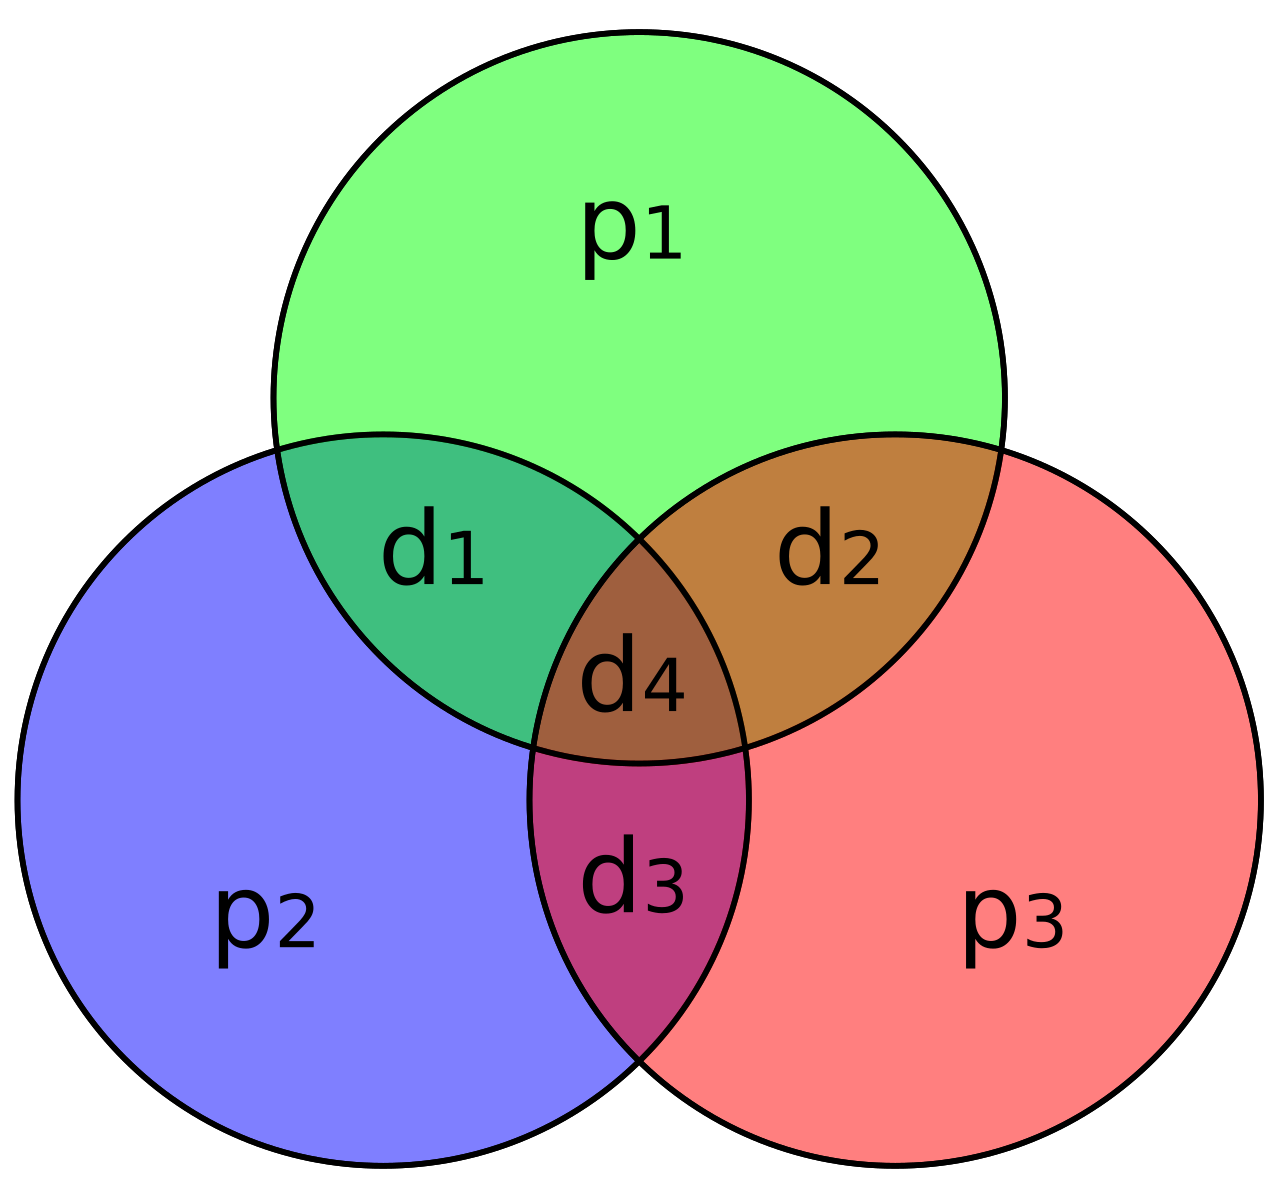
\includegraphics[width=7cm, height=4cm, keepaspectratio]{figures/Hamming(7,4).png}      
    
    \caption{The Hamming(7,4) code (with r = 3)}
    \label{fig:fig1}
\end{figure*}
\section{Objective ,Methodology and Implementation}
\subsection{OBJECTIVE-I : Hamming Code Algorithm}
\subsubsection{Code Layout}
Encode 8-bit data into a 12-bit code word.\\
Compute parity bits to ensure error detection and correction.\\
Include error detection and single-bit error correction for the receiving Arduino.\\
\textbf{Bit positions: }
The 12-bit Hamming code is structured as follows:

   \begin{table}[h!]
    \centering
    \caption{Hamming (12,8) Code Layout}

    \begin{tabular}{|c|c|c|c|c|c|c|c|c|c|c|c|c|}
        \hline
        \textbf{Bit Position} & 12 & 11 & 10 & 9 & 8 & 7 & 6 & 5 & 4 & 3 & 2 & 1 \\
        \hline
        \textbf{Bit Type} & D8 & D7 & D6 & D5 & P8 & D4 & D3 & D2 & P4 & D1 & P2 & P1 \\
        \hline
    \end{tabular}
   
\end{table}
       \noindent  D1 to D8 are the 8 data bits.\\
        P1, P2, P4, and P8 are the 4 parity bits. \cite{attarian2006coding}

\subsubsection{Designing the Hamming Code}
\begin{itemize}

\item {Step 1: Determine the number of parity bits.}
Given a data bit sequence of length \(m\), the number of parity bits \(r\) is determined such that:
\begin{equation}
2^r \geq m + r + 1
\end{equation}

\item  {Step 2: Position the parity bits}
Place the parity bits at positions that are powers of 2 (i.e., positions 1, 2, 4, 8, etc.). The remaining positions are reserved for data bits.

\item {Step 3: Calculate parity bit values,}
The value of each parity bit is calculated based on specific bits in the data sequence. For each parity bit, cover bits are determined using binary representation. For example, parity bit \(P_1\) covers bits at positions where the least significant bit of their binary representation is 1.

\textbf{Example}Consider a 4-bit data sequence: \texttt{1011}.

\begin{enumerate}
    \item Calculate the number of parity bits needed:
    \begin{equation}
    2^r \geq 4 + r + 1 \implies r = 3
    \end{equation}
    \item Insert parity bits at positions 1, 2, and 4: \texttt{P1, P2, 1, P4, 0, 1, 1}.
    \item Calculate values for each parity bit:
    \begin{itemize}
        \item \(P_1\) covers positions 1, 3, 5, 7.
        \item \(P_2\) covers positions 2, 3, 6, 7.
        \item \(P_4\) covers positions 4, 5, 6, 7.
    \end{itemize}
\end{enumerate}
A (12,8) Hamming code uses 8 data bits and 4 parity bits to form a 12-bit code word. The parity bits are strategically placed in positions that are powers of two (1, 2, 4, and 8), while the data bits are placed in the remaining positions.\cite{khadir}
\end{itemize}
\subsubsection{Types of Hamming Code Algorithms}

Hamming code is a family of error-detecting and error-correcting codes that can correct single-bit errors and detect two-bit errors. Below are the common types of Hamming codes:

\begin{enumerate}

\item \textbf{(7,4) Hamming Code}

The (7,4) Hamming Code is one of the simplest and most commonly used Hamming codes. It takes 4 data bits and adds 3 parity bits to form a 7-bit codeword. The extra bits enable error detection and correction. The algorithm for encoding and decoding is as follows:

\item \textbf{(15,11) Hamming Code}

The (15,11) Hamming Code is an extended version that encodes 11 data bits into a 15-bit codeword by adding 4 parity bits. This increases error detection and correction capabilities.
\item \textbf{Generalized Hamming Code}

The generalized Hamming code is a more flexible version of the Hamming code that can be used for different block sizes and error-correcting capabilities.
\item \textbf{Extended Hamming Code}

Extended Hamming codes are derived by adding an extra parity bit to the standard Hamming codes, enabling detection of two-bit errors. 
\end{enumerate}

\pagebreak
\subsection{OBJECTIVE-II : Implementing on software}

\textbf{Function to Encode and Decode Hamming code}

Below is a simple C++ function to implement a Hamming code encoding and decoding algorithm:\cite{beneater2018}


\begin{tabular}{cc}

\textbf{Encoding Algorithm} & \textbf{Decoding Algorithm} \\
       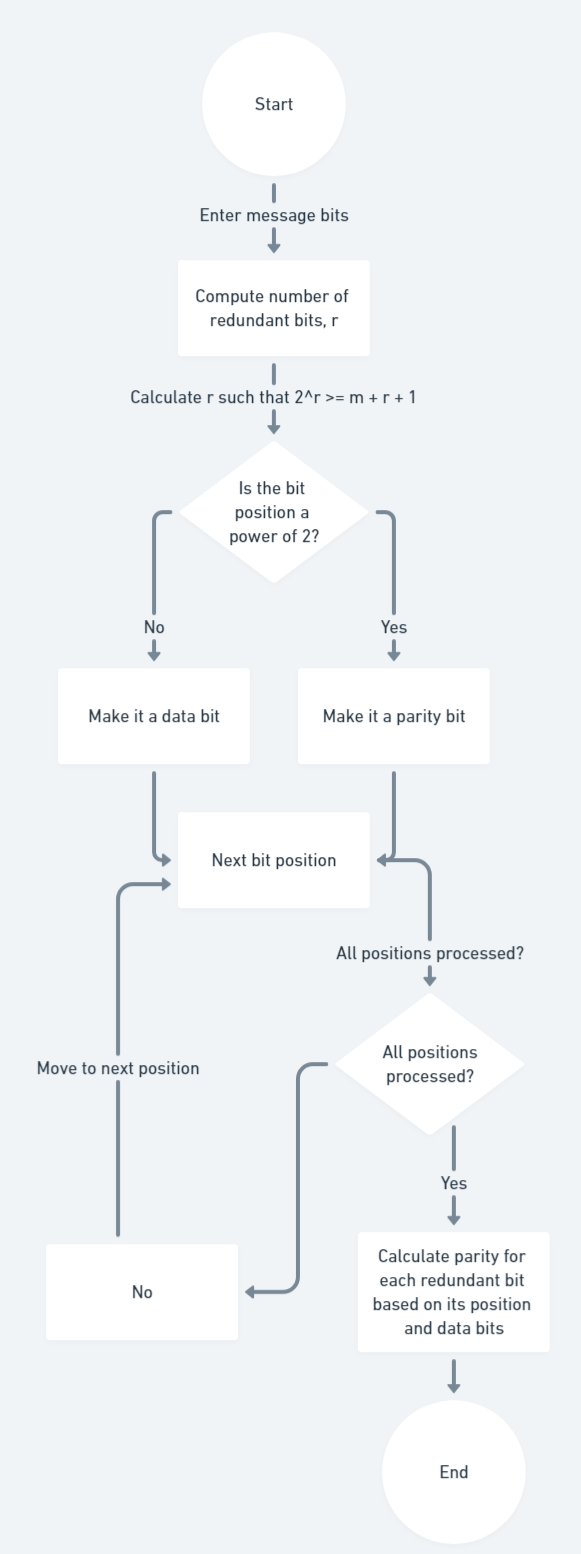
\includegraphics[scale=0.545]{encoding.png} 
       &
       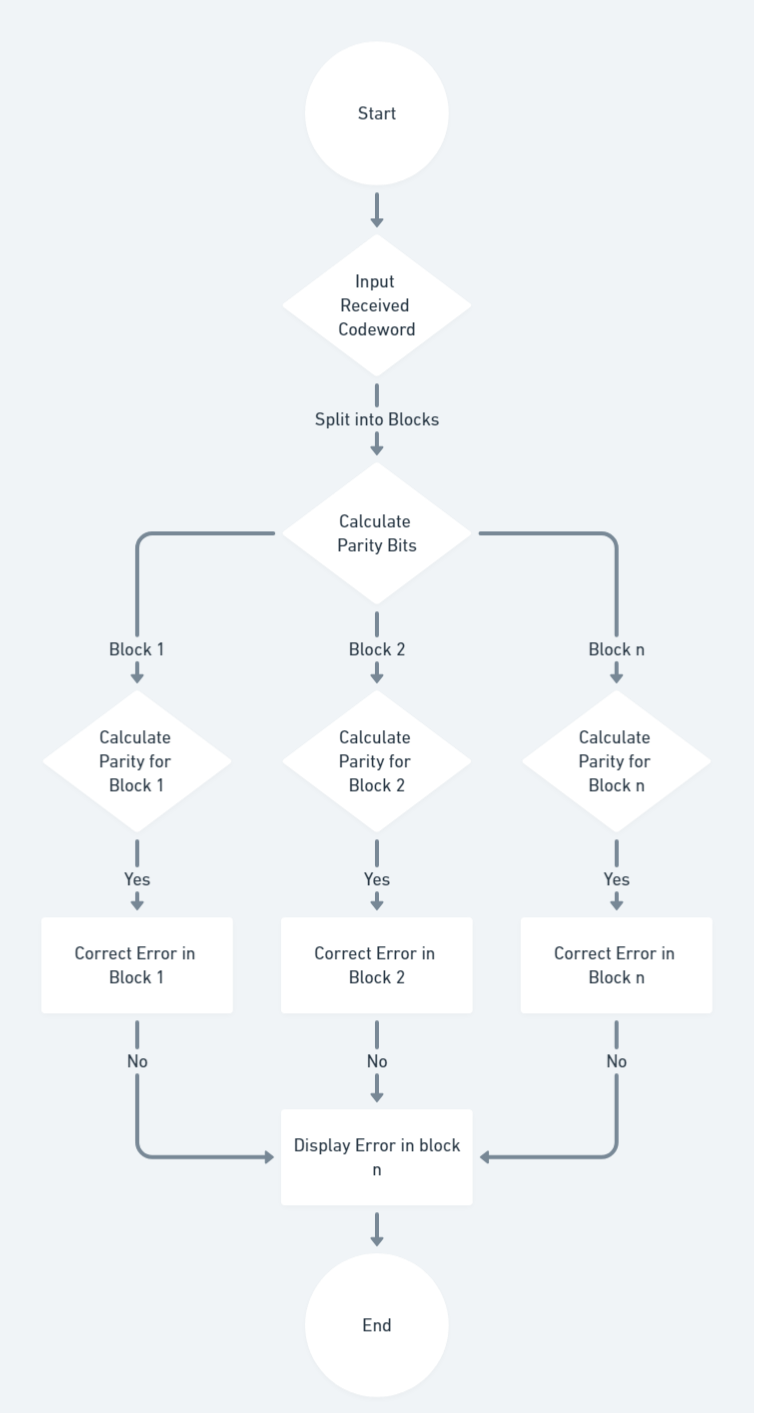
\includegraphics[scale=0.6]{decoding.png}\\
\end{tabular}

\centerline{Figure 4.1(a): Encoding flow diagram \& 4.1(b): Decoding flow diagram}
% \begin{minipage}{0.45\textwidth}
%     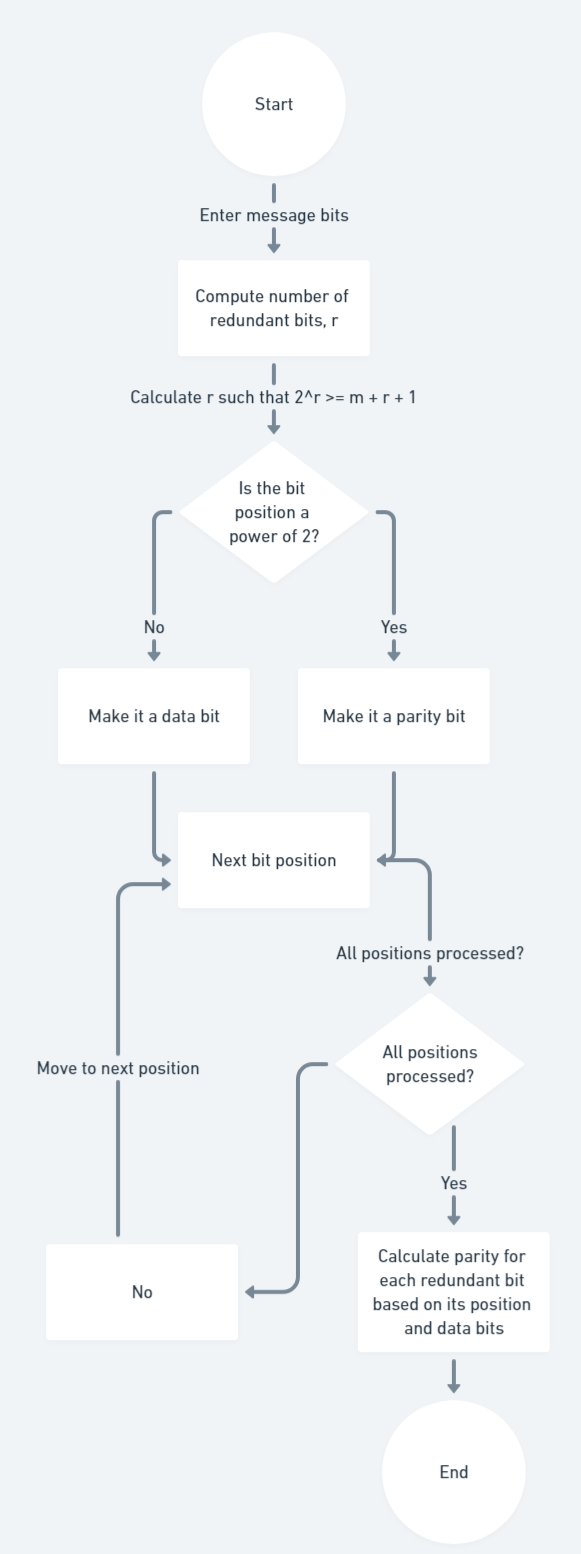
\includegraphics[scale=0.5]{encoding.png}
   
% \end{minipage}
% \hfill
% \begin{minipage}{0.45\textwidth}
%     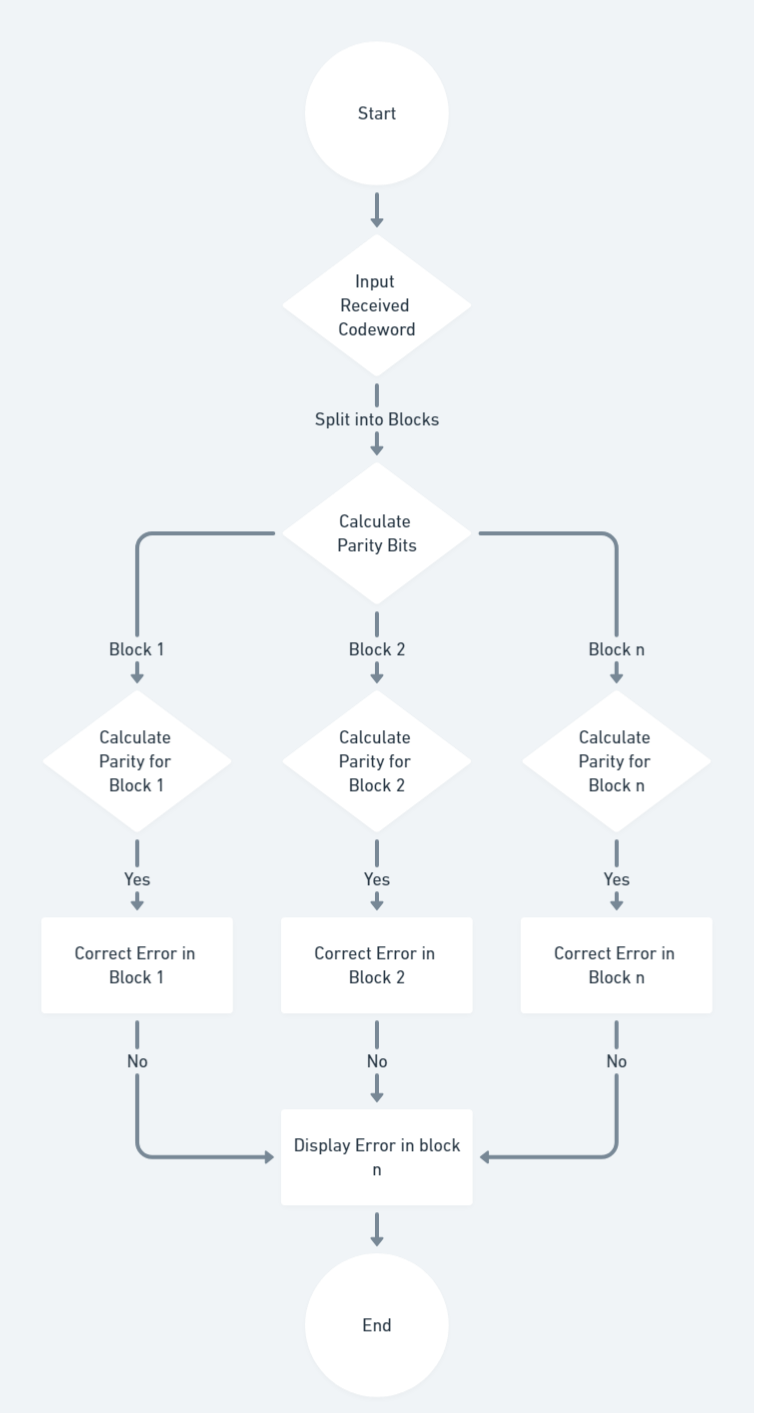
\includegraphics[scale=0.5]{decoding.png}
   
% \end{minipage}





 %   \subsection{Encoding Function}

 %       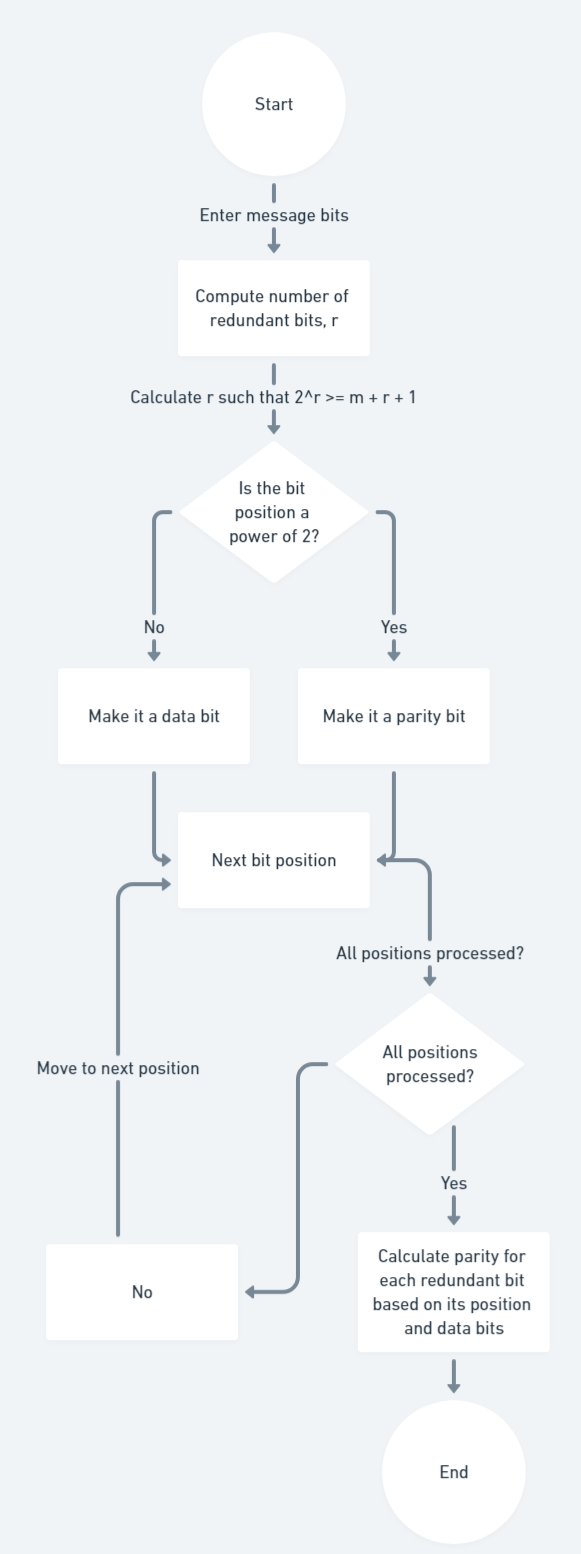
\includegraphics[width=0.3\linewidth]{encoding.png}
 
    
 % \subsection{Decoding Function}

 %    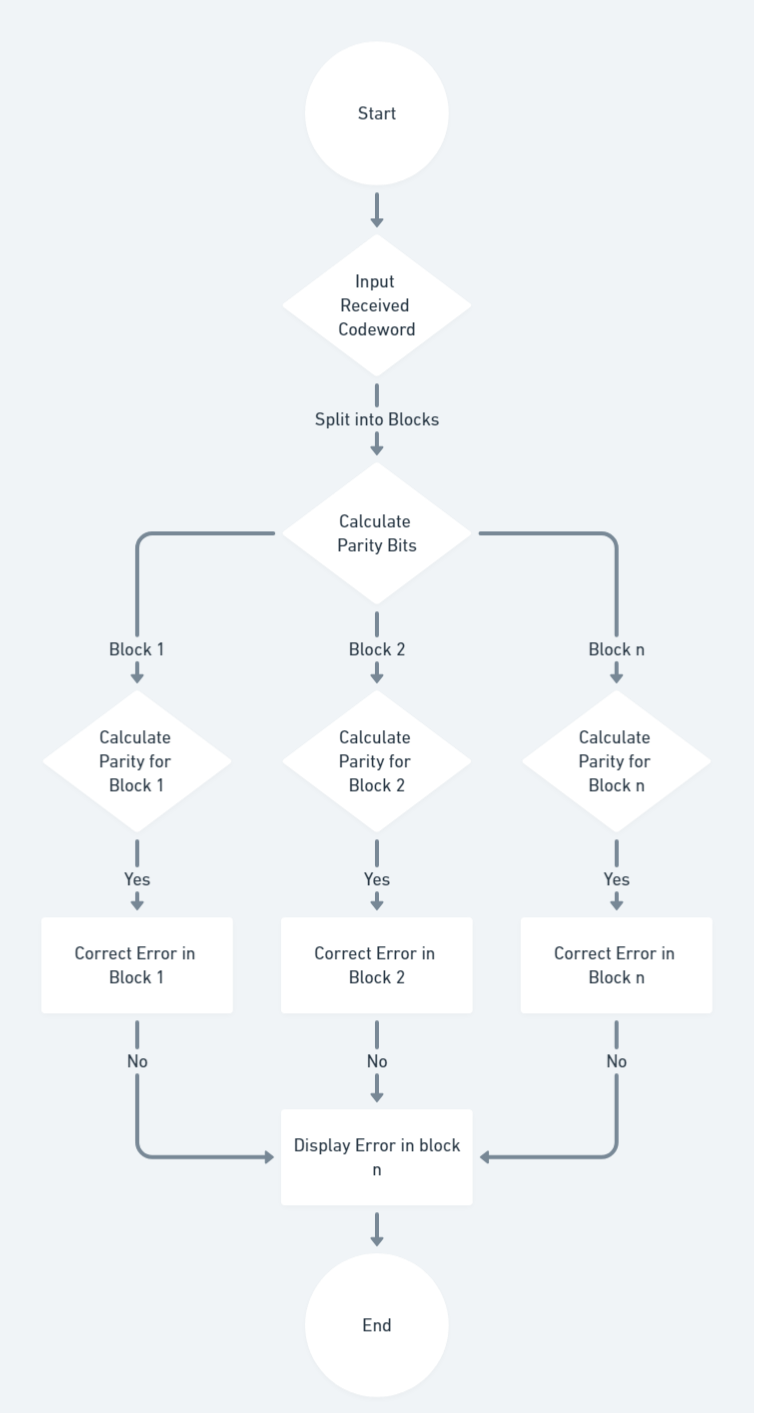
\includegraphics[width=0.5\linewidth]{decoding.png}


\subsection{OBJECTIVE-III : Implementing on Microprocessor}
Implement the Hamming (12,8) code encoding and decoding on a microprocessor, such as an Arduino. This implementation will allow real-time error detection and correction in data transmitted between devices.
\begin{enumerate}
    \item {Setting Up the Microprocessor}
        \begin{itemize}
        \item Use an Arduino (or similar micro controller) to send and receive data.
        \item Connect the Arduinos via Serial or I2C communication, which allows them to send and receive data reliably.
        \end{itemize}
    \item{Programming the Encoder and Decoder}
    \begin{itemize}
        \item Write functions to encode 8-bit data into a 12-bit Hamming code.
        \item Write functions to decode the 12-bit Hamming code back into 8-bit data and correct single-bit errors if necessary.
    \end{itemize}
    \item {Integrating the Hamming Encoder and Decoder Code}
    \begin{itemize}
    \item Import the encoder and decoder header files into your Arduino sketch.
    \item Designate one Arduino as the \textbf{transmitter} (encoding and sending data) and the other as the \textbf{receiver} (decoding and error-checking the received data).
    \end{itemize}
\end{enumerate}

\textbf {Tools for Hamming Code Implementation on an Arduino}
\begin{table}[h!]
\caption{Tools for Hamming code Implementation}
\label{tab:5.1}
\begin{tabular}{|l|p{13cm}|}
\hline
\textbf{Tool} & \textbf{Description} \\
\hline
Arduino Board & The microcontroller board ie, Arduino nano using ATmega32P used for coding and testing the Hamming Code implementation. \\
\hline
Arduino IDE & Software used to write, compile, and upload code to the Arduino board. It provides an environment for developing Hamming code logic in C/C++. \\
\hline
Breadboard & Used for building and testing the circuit without soldering, connecting the Arduino pins with peripherals like LEDs and switches. \\
\hline
Jumper Wires & Used to make connections between the Arduino, breadboard, and other components in the circuit. \\
\hline
LEDs & Can be used as output indicators for testing Hamming code output such as error detection/correction results. \\
\hline
Resistors & Typically used with LEDs to limit current and protect components during testing and debugging. \\
\hline
Oscilloscope & A device used to observe and analyze the electrical signals in the circuit, which is helpful for debugging timing and signal integrity issues. \\
\hline
PS/2 Keyboard & A peripheral device that can be used for input testing and interfacing with the Arduino to send data streams that may require Hamming code error checking. \\
\hline
\end{tabular}

\end{table}

\pagebreak
\subsection{Implementation Steps}
\begin{enumerate}

\item \textbf{Software Implementation}

Writing a program to encode data into Hamming code and decode the same. 
This involves:
\begin{itemize}
    \item Implementing algorithms for data encoding, parity bit generation, and error detection.
    \item Introducing controlled random bit flips to simulate data corruption during transmission.
    \item Decoding the corrupted data and applying error correction techniques to restore the original message.
    \item Testing with various message lengths and error scenarios to validate robustness.
\end{itemize}
The software implementation ensures that the Hamming code performs well under simulated transmission errors, making the data error-free.

\item \textbf{Implementation Between Two Communicating Arduinos}

Establishing a reliable communication link between two Arduino microcontrollers involves:
\begin{itemize}
    \item Configuring one Arduino as a transmitter and the other as a receiver.
    \item Using serial communication protocols (e.g., UART or I2C) to transmit data.
    \item Encoding data at the transmitter using Hamming code and decoding it at the receiver to detect and correct errors.
    \item Simulating environmental noise or interference to induce random errors during transmission.
    \item Validating data integrity at the receiver and displaying results on an LCD or serial monitor.
\end{itemize}
This implementation demonstrates practical error correction in embedded systems.

\item \textbf{Implementation on a Microprocessor}

Building a transmitter and a receiver on a microprocessor platform includes:
\begin{itemize}
    \item Developing separate routines for encoding data into Hamming code at the transmitter and decoding it at the receiver.
    \item Interfacing input devices (e.g., keyboards or sensors) to provide data to the transmitter.
    \item Connecting output devices (e.g., LCDs or LEDs) to display decoded data and error correction results.
    \item Optimizing the microprocessor code to handle large data sets and ensure minimal latency in encoding/decoding processes.
    \item Testing performance under different operating conditions, such as high data rates or noisy environments.
\end{itemize}
The microprocessor-based implementation showcases the adaptability of Hamming code for real-world applications.

% \item \textbf{Future Enhancements and Applications}

% Exploring possible enhancements and applications of Hamming code:
% \begin{itemize}
%     \item Improving the error correction capability by integrating advanced techniques like Reed-Solomon or BCH codes.
%     \item Implementing Hamming code in wireless communication systems to ensure data integrity over long distances.
%     \item Using Hamming code in storage devices to prevent data corruption during read/write operations.
%     \item Integrating Hamming code with IoT devices for secure and reliable data exchange in smart systems.
%     \item Exploring hardware-based implementations using FPGA or ASIC for high-speed applications.
% \end{itemize}
% These advancements will expand the utility of Hamming code in modern digital systems.

\end{enumerate}
\pagebreak
\subsection{Methodology}
 \subsubsection{Thought Train Mapping}
    \begin{figure*}[!ht]
    \centering
    
    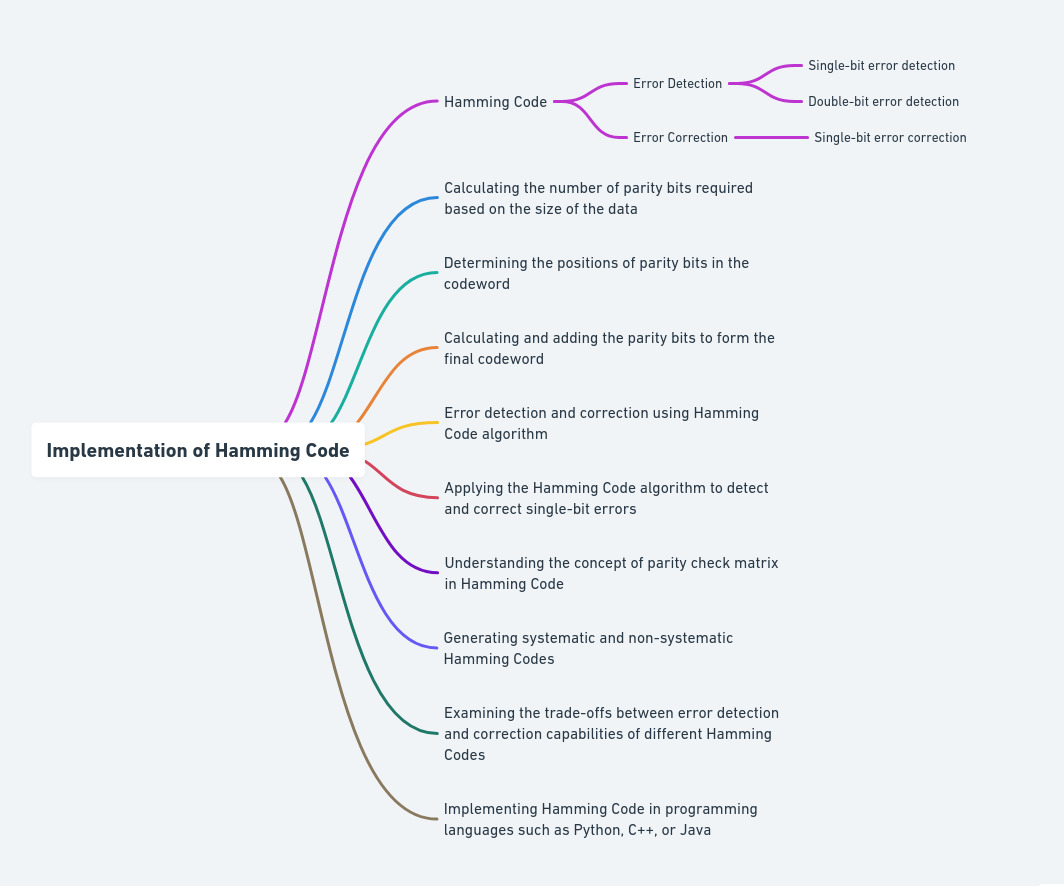
\includegraphics[width=20cm, height=10cm, keepaspectratio]{figures/flow1.jpeg}      
    
    \caption{Methodology Mindmap}
    \label{fig:fig2}
\end{figure*}
    
 \subsubsection{System design Mapping}
    \begin{figure*}[!ht]
    \centering
    
    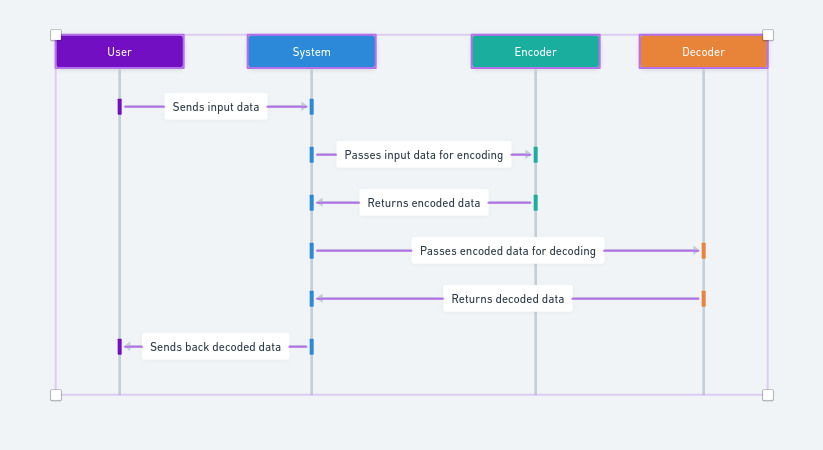
\includegraphics[width=14cm, height=8cm, keepaspectratio]{figures/system_design.jpeg}      
    
    \caption{Algorithim Sequence flow}
    \label{fig:fig3}
\end{figure*}

\pagebreak
\subsubsection{Technologies Used}
\subsubsection {Overview of PS 2}  
The PS/2 keyboard is a type of input device that connects to a computer through the PS/2 port, a standard interface developed by IBM in 1987. This keyboard and connector were widely used in earlier computer systems but have been largely replaced by USB interfaces.\cite{ps2}

\textbf{PS/2 Connector}
      
       
       \label{fig:fig4}
\begin{figure}[htbp]
    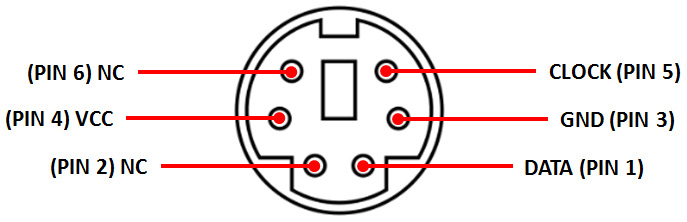
\includegraphics[width=0.5\linewidth]{WhatsApp Image 2024-12-02 at 12.30.14 PM.jpeg}
    \centering
    \caption{PS/2 connector Pin diagram}
    \label{fig:fig4}
\end{figure}
    

The PS/2 connector is a 6-pin mini-DIN connector with the following characteristics:
\begin{itemize}
    \item \textbf{Round Design}: The connector has a circular shape with six metal pins and a keyway for orientation.
    \item \textbf{Pin Configuration}: Each pin has a specific function:
    \begin{itemize}
        \item \textbf{Pin 1}: Data
        \item \textbf{Pin 2}: Reserved
        \item \textbf{Pin 3}: Ground
        \item \textbf{Pin 4}: +5V (Power)
        \item \textbf{Pin 5}: Clock
        \item \textbf{Pin 6}: Reserved
    \end{itemize}
    \item \textbf{Data Transmission}: Communication occurs synchronously, with the keyboard generating clock signals for data transmission.
\end{itemize}
\pagebreak
\textbf{Table for keyboard scan codes}\\

\begin{figure}[htbp]
    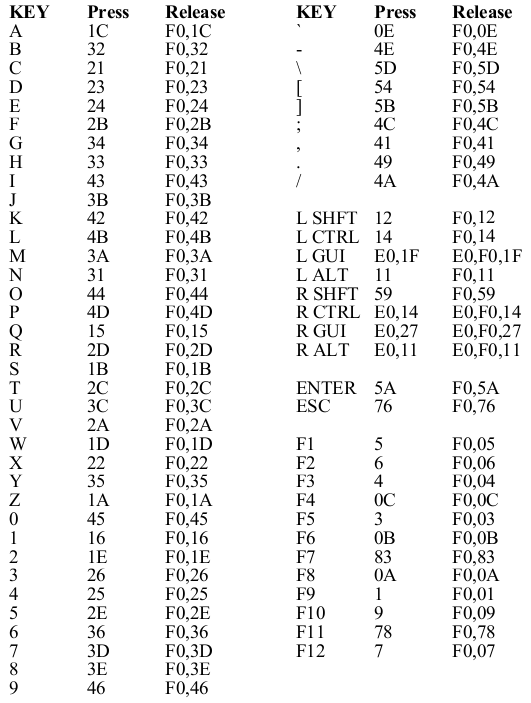
\includegraphics[width=10cm, keepaspectratio]{theps2protocol_1236112658.png}
    \centering
    \caption{Scan Codes}
    \label{fig:fig5}
\end{figure}

\texbf{Advantages and Disadvantages}
\textbf{Advantages}
\begin{itemize}
    \item Supports lower latency compared to USB keyboards.
    \item Allows ``n-key rollover,'' enabling simultaneous key presses without ghosting.
\end{itemize}

\textbf{Disadvantages}
\begin{itemize}
    \item Does not support hot-plugging. Connecting or disconnecting a device while the system is powered on may cause issues.
    \item The interface is becoming obsolete as USB has become the new standard.
\end{itemize}

\subsubsection{Overview of interrupts in Arduino}
Interrupts in Arduino allow the microcontroller to stop its current task and execute a specific block of code when a certain event occurs. This is particularly useful for time-sensitive tasks or when dealing with asynchronous inputs like sensors or user inputs.

Interrupts in Arduino allow the microcontroller to temporarily halt its current task and execute a predefined block of code in response to specific events or conditions. When an interrupt occurs, the microcontroller's normal operation is paused, and it jumps to a special function called an interrupt service routine (ISR) to handle the event. After the ISR completes, the microcontroller returns to its previous task. This mechanism is crucial for handling time-sensitive tasks or responding to asynchronous events in real-time without continuously checking for them in the main program loop.

\textbf{Types of Interrupts in Arduino}
Arduino supports the following types of interrupts:
\begin{itemize}
    \item \textbf{External Interrupts:} Triggered on specific pins (e.g., \texttt{INT0}, \texttt{INT1}) on most Arduino boards.
    \item \textbf{Pin Change Interrupts:} Available on all pins, but their implementation is less direct.
\end{itemize}

\textbf{Commonly Used Interrupt Modes}
\begin{itemize}
    \item \texttt{LOW}: Triggered when the pin is low.
    \item \texttt{CHANGE}: Triggered when the pin changes state.
    \item \texttt{RISING}: Triggered when the pin transitions from LOW to HIGH.
    \item \texttt{FALLING}: Triggered when the pin transitions from HIGH to LOW.
\end{itemize}

\textbf{Syntax for Using Interrupts}
The function \texttt{attachInterrupt()} is used to configure and enable interrupts on Arduino.

\begin{lstlisting}[caption={Syntax for attachInterrupt}]
attachInterrupt(digitalPinToInterrupt(pin), ISR, mode);
\end{lstlisting}

\begin{description}
    \item[\texttt{pin}]: The pin number to attach the interrupt to.
    \item[\texttt{ISR}]: The Interrupt Service Routine, a function that runs when the interrupt is triggered.
    \item[\texttt{mode}]: The condition that triggers the interrupt (e.g., \texttt{RISING}, \texttt{FALLING}, \texttt{CHANGE}, \texttt{LOW}).
\end{description}


\textbf{Important Notes}
\begin{itemize}
    \item The \textbf{Interrupt Service Routine (ISR)} should be kept as short and efficient as possible to avoid delays in other tasks.
    \item Functions like \texttt{delay()}, \texttt{Serial.print()}, or other time-consuming operations are not recommended inside an ISR.
    \item Use the \texttt{volatile} keyword for variables shared between the ISR and the main program to prevent compiler optimizations.
\end{itemize}

\subsubsection{Overview of LCD}
Liquid Crystal Displays (LCDs) are flat-panel displays that utilize the light-modulating properties of liquid crystals combined with a backlight or reflector to produce images. They are widely used in devices such as televisions, computer monitors, mobile phones, and more.\cite{lcd}
\begin{figure}[htbp]
    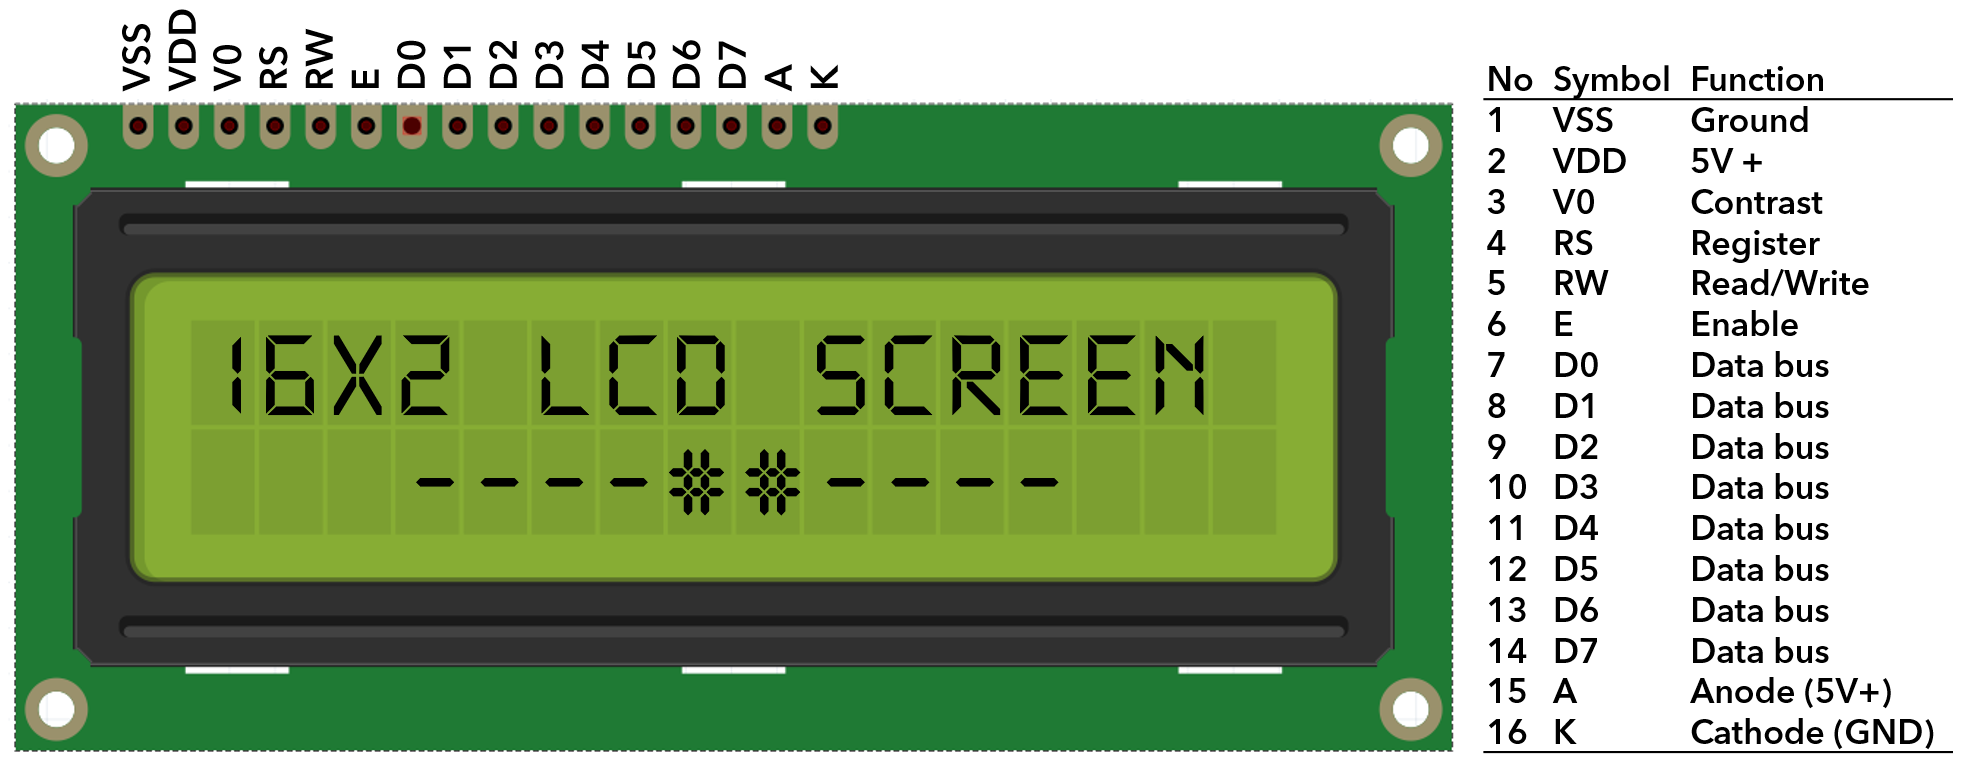
\includegraphics[width=10cm, keepaspectratio]{16X2-LCD-PINS.PNG}
    \centering
    \caption{Scan Codes}
    \label{fig:fig5}
\end{figure}

\textbf{Working Principle}
The operation of an LCD is based on the ability of liquid crystals to control the passage of light. Key components include:
\begin{itemize}
    \item \textbf{Liquid Crystal Material:} Changes its optical properties when an electric field is applied.
    \item \textbf{Polarizing Filters:} Ensure that only light aligned in certain directions passes through.
    \item \textbf{Electrodes:} Create the electric field to manipulate liquid crystals.
\end{itemize}
The combination of these components allows LCDs to display images by selectively blocking or allowing light to pass through.

\textbf{Types of LCDs}
There are various types of LCDs, categorized based on their technology and application:
\begin{itemize}
    \item \textbf{Twisted Nematic (TN):} Known for fast response times and low cost.
    \item \textbf{In-Plane Switching (IPS):} Offers better color reproduction and viewing angles.
    \item \textbf{Vertical Alignment (VA):} Provides high contrast ratios.
\end{itemize}

\textbf{Advantages}
\begin{itemize}
    \item Low power consumption compared to older display technologies.
    \item Lightweight and slim design.
    \item High resolution and image quality.
\end{itemize}

\textbf{Applications}
LCDs are used in a wide range of devices, including:
\begin{itemize}
    \item Smartphones
    \item Laptops
    \item Televisions
    \item Digital clocks
    \item Instrument panels
\end{itemize}

\textbf{Challenges and Limitations}
While LCDs are popular, they also have certain drawbacks:
\begin{itemize}
    \item Limited viewing angles (improved in IPS technology).
    \item Dependency on backlight reduces contrast compared to OLEDs.
    \item Potential for motion blur in fast-moving images.
\end{itemize}




\subsection{USART Overview}
The Universal Asynchronous Receiver-Transmitter (USART) protocol is one of the simplest and most widely used methods for serial data communication. USART operates asynchronously, meaning it does not require a clock signal for data transmission. Instead, it relies on a pre-defined baud rate (speed of transmission) and synchronization between the transmitter and receiver.

Although USART is often considered an older communication method, it continues to play a crucial role in modern electronics. Its simple implementation, low cost, and widespread support make it suitable for a wide range of applications, from microcontroller-based systems to peripheral communication in computers and industrial systems.

In this document, we explore the various aspects of the USART protocol, from its basic functioning to its use in modern devices. We will cover its data format, the components involved, and the communication process in detail.\cite{usart}
\begin{figure}[htbp]
    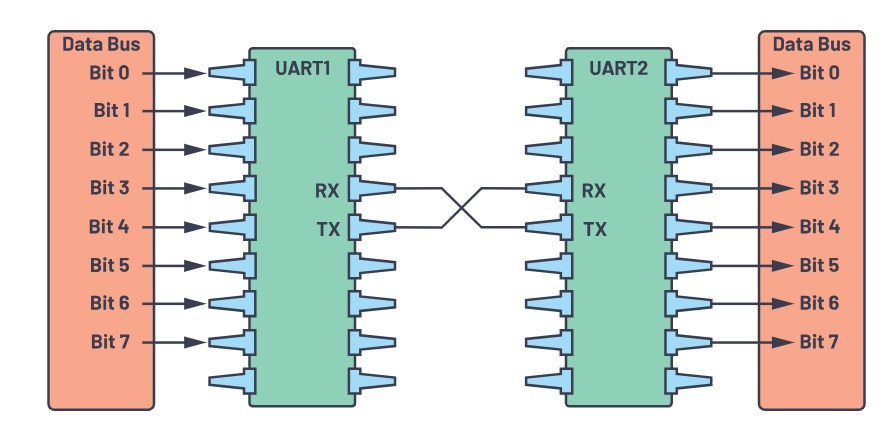
\includegraphics[width=0.8\linewidth]{WhatsApp Image 2024-12-02 at 2.04.51 PM.jpeg}
    \centering
    \caption{USART diagram}
    \label{fig:fig7}
\end{figure}


\textbf{Basic Operation of USART}
At the core of USART is the process of transmitting and receiving data bit-by-bit through a single communication line. Data is sent asynchronously, meaning there is no need for a clock signal to synchronize the data transmission. Instead, both the transmitter and receiver must operate at the same baud rate.

A basic USART communication cycle involves the following stages:

\begin{enumerate}
    \item \textbf{Start Bit:} The start bit marks the beginning of data transmission. It is a low logic level (0) and is sent before the actual data bits to alert the receiver that new data is coming. The start bit ensures that the receiver is ready to receive the incoming data.
    
    \item \textbf{Data Bits:} After the start bit, the data bits follow. The number of data bits is usually 8, though USART supports configurations with 5 to 9 bits per character. These bits represent the actual data being transmitted. The data bits are sent one by one in sequence from the least significant bit (LSB) to the most significant bit (MSB).
    
    \item \textbf{Parity Bit (Optional):} The parity bit is an optional error-checking mechanism. It can be configured to be even, odd, or none. When used, the parity bit is calculated based on the number of 1s in the data bits. In even parity, the number of 1s in the data bits, plus the parity bit, must be even, while in odd parity, the total number of 1s must be odd.
    
    \item \textbf{Stop Bits:} Stop bits signal the end of the data transmission. These bits are set to a high logic level (1) and ensure that the receiver knows when the transmission of one byte is complete. One or two stop bits are typically used in most configurations.
\end{enumerate}

\textbf{Baud Rate:} The baud rate determines the speed at which data is transmitted and received. It is typically expressed in bits per second (bps). Common baud rates include 9600, 19200, 38400, and 115200 bps. Both the transmitter and receiver must operate at the same baud rate for successful communication.

\textbf{USART Data Format}
The USART protocol defines a standard format for sending and receiving data. As mentioned earlier, the basic USART data format consists of the start bit, data bits, an optional parity bit, and stop bits. Below is a breakdown of the typical USART frame structure:

\begin{itemize}
    \item \textbf{Start Bit:} A single low bit (0) indicating the beginning of data transmission.
    \item \textbf{Data Bits:} The data being transmitted. This usually consists of 8 bits, but can range from 5 to 9 bits.
    \item \textbf{Parity Bit (optional):} An optional bit used for error checking. The parity bit helps detect transmission errors by ensuring that the number of 1s in the data is either even or odd, depending on the configuration.
    \item \textbf{Stop Bits:} One or more bits (usually 1 or 2) set to a high logic level (1) to indicate the end of the transmission. These bits give the receiver enough time to process the data and get ready for the next transmission.
\end{itemize}

The configuration of these parameters (data bits, parity, and stop bits) can be customized depending on the requirements of the communication system. For instance, the number of data bits can be adjusted to fit different types of data, and parity can be enabled to ensure error detection.

\textbf{Error Detection in USART}
While USART is a simple protocol, it does provide basic mechanisms for error detection. These mechanisms help ensure that data is transmitted correctly and that errors can be identified and corrected.

\subtextbf{Parity Bit}
The parity bit is the most basic form of error detection in USART. It is used to verify whether the transmitted data has been received correctly. There are two main types of parity:
\begin{itemize}
    \item \textbf{Even Parity:} The parity bit ensures that the total number of 1s in the data (including the parity bit) is even.
    \item \textbf{Odd Parity:} The parity bit ensures that the total number of 1s in the data (including the parity bit) is odd.
\end{itemize}
If the number of 1s in the data does not match the expected parity (even or odd), an error is detected, and the data is flagged as corrupt.

\textbf{Stop Bit Monitoring}
Another basic form of error detection is the monitoring of stop bits. If the stop bit is not at a high logic level (1), the receiver may interpret this as an error and discard the data.

\textbf{Flow Control in USART}
Flow control is used to manage the rate at which data is transmitted to ensure that the receiver can process the incoming data without losing any information. USART supports two types of flow control:

\textbf{Hardware Flow Control (RTS/CTS)}
Hardware flow control uses additional wires, typically \textit{Request to Send} (RTS) and \textit{Clear to Send} (CTS), to signal when the receiver or transmitter is ready to transmit or receive data. This method ensures that data is only transmitted when the receiver is ready, preventing data loss.

\textbf{Software Flow Control (XON/XOFF)}
Software flow control uses control characters (XON and XOFF) to manage data transmission. When the receiver's buffer is full, it sends the XOFF character to instruct the transmitter to pause transmission. Once the receiver is ready, it sends the XON character to resume data flow.

\textbf{Applications of USART}
USART is a versatile protocol used in a variety of applications. Some common uses include:

\begin{itemize}
    \item \textbf{Microcontrollers:} USART is widely used for communication between microcontrollers and external peripherals like sensors, displays, and actuators.
    \item \textbf{Computer Peripherals:} USART is used in devices like modems, GPS receivers, Bluetooth modules, and other communication peripherals.
    \item \textbf{Embedded Systems:} USART is a standard communication protocol in embedded systems for serial communication with external devices.
    \item \textbf{Networking:} Although it is not used for high-speed networking, USART can be used for lower-speed data communication, such as in RS-232 and RS-485 networks.
\end{itemize}

\textbf{Advantages of USART}
The USART protocol offers several advantages:


\begin{itemize}
    \item \textbf{Simplicity:} USART is a simple protocol that requires minimal hardware and software support.
    \item \textbf{Low Cost:} The protocol's minimal hardware requirements make it cost-effective for many applications.
    \item \textbf{Asynchronous Communication:} USART does not require a clock signal, simplifying system design and reducing the number of required pins.
    \item \textbf{Wide Adoption:} USART is widely supported by microcontrollers and other embedded devices, making it easy to integrate into a variety of systems.
\end{itemize}



\pagebreak
\section{\centering Results \& Discussion}
Results of the above objective were sequentially achieved and Realized.
\subsection{Result of Objective-I}
\textbf{Implementation of the Hamming code encoder in C++ steps:}

% \begin{lstlisting}[language=C++,title=code snippet 1: Hamming Code Encoding]
% void Hamm_conv(int tx_data[8])
% { 
%   int parity[4];
%   int i=0;
%   int j=0;
%   int c=0;
  
%   parity[0]=tx_data[0]^tx_data[1]^tx_data[3]^tx_data[4]^tx_data[6];
%   parity[1]=tx_data[0]^tx_data[2]^tx_data[3]^tx_data[5]^tx_data[6];
%   parity[2]=tx_data[1]^tx_data[2]^tx_data[3]^tx_data[7];
%   parity[3]=tx_data[4]^tx_data[5]^tx_data[6]^tx_data[7];

%   while(i<12)
%   {
%     if(i==0||i==1||i==3||i==7)
%     { hamm[i] = parity[j];
%       j++;
%       i++;
%     }
%     else{
%       hamm[i]=tx_data[c];
%       c++;
%       i++;
%     } 
%   }  
% }
% \end{lstlisting}

\textbf{Algorithim for Hamming code Encoder}
\begin{enumerate}
    \item \textbf{Input Data Bits}: Take $k$ data bits from the user.
    \item \textbf{Determine Number of Parity Bits}: Calculate $r$ such that $2^r \geq k + r + 1$.
    \item \textbf{Position Data and Parity Bits}:
          \begin{itemize}
              \item Create a combined array of size $n = k + r$.
              \item Place parity bits at positions that are powers of 2 ($1, 2, 4, 8, \ldots$).
              \item Place data bits in the remaining positions.
          \end{itemize}
    \item \textbf{Calculate Parity Bits}:
          \begin{itemize}
              \item For each parity bit position $2^{i-1}$, compute parity using XOR of all covered positions.
          \end{itemize}
    \item \textbf{Output Hamming Code}: Print the combined array as the encoded Hamming code.
\end{enumerate}


\textbf{Algorithim for Hamming code Encoder} 
\begin{enumerate}
    \item \textbf{Input the Received Code}: Take the $n$-bit received Hamming code from the user.
    \item \textbf{Determine the Number of Parity Bits}:
          \begin{itemize}
              \item Calculate $r$ (number of parity bits) such that $2^r \geq n + 1$.
          \end{itemize}
    \item \textbf{Check Parity Bits}:
          \begin{itemize}
              \item Compute the parity at each $2^{i-1}$ position by XORing all bits covered by that parity bit.
              \item Store the results in a binary number called the \textit{syndrome}.
          \end{itemize}
    \item \textbf{Detect and Correct Errors}:
          \begin{itemize}
              \item If the syndrome is non-zero, it indicates an error at the position corresponding to the binary value of the syndrome.
              \item Flip the bit at the error position to correct the code.
          \end{itemize}
    \item \textbf{Extract the Data Bits}:
          \begin{itemize}
              \item Remove all parity bit positions ($2^{i-1}$) from the corrected code to retrieve the original data bits.
          \end{itemize}
\end{enumerate}














% \begin{lstlisting}[language=C++, title =code snippet 2: Hamming Code decoding]
%  int decode_hamming(int en_msg[]){
%  int P1 = (en_msg[11]) & 1;
%  int P2 = (en_msg[10]) & 1;
%  int D1 = (en_msg[9]) & 1;
%  int P4 = (en_msg[8]) & 1;
%  int D2 = (en_msg[7]) & 1;
%  int D3 = (en_msg[6]) & 1;
%  int D4 = (en_msg[5]) & 1;
%  int P8 = (en_msg[4]) & 1;
%  int D5 = (en_msg[3]) & 1;
%  int D6 = (en_msg[2]) & 1;
%  int D7 = (en_msg[1]) & 1;
%  int D8 = (en_msg[0]) & 1; 
%   // Calculate the Par bits
%   // injecting error
%   D8^=1;
%   int C1 = P1 ^ D1 ^ D2 ^ D4 ^ D5 ^ D7;
%   int C2 = P2 ^ D1 ^ D3 ^ D4 ^ D6 ^ D7;
%   int C4 = P4 ^ D2 ^ D3 ^ D4 ^ D8;
%   int C8 = P8 ^ D5 ^ D6 ^ D7 ^ D8;
%   int errorPos = (C8 << 3) | (C4 << 2) | (C2 << 1) | C1;
%   if (errorPos != 0) {
%     Serial.println("error at");
%     Serial.println(errorPos);
%     en_msg[errorPos-1]^=1;
%   }
%   else{
%     Serial.println("no error");
%   }
%   P1 = (en_msg[11]) & 1;
%   P2 = (en_msg[10]) & 1;
%   D1 = (en_msg[9]) & 1;
%   P4 = (en_msg[8]) & 1;
%   D2 = (en_msg[7]) & 1;
%   D3 = (en_msg[6]) & 1;
%   D4 = (en_msg[5]) & 1;
%   P8 = (en_msg[4]) & 1;
%   D5 = (en_msg[3]) & 1;
%   D6 = (en_msg[2]) & 1;
%   D7 = (en_msg[1]) & 1;
%   D8 = (en_msg[0]) & 1;
  
%   // Extract the original 8 data bits
%   int decodedData = (D1 << 0) | (D2 << 1) | (D3 << 2) | (D4 << 3) | (D5 << 4) | (D6 << 5) | (D7 << 6) | (D8 << 7);
  
%   return decodedData;
% }
% \end{lstlisting}

\subsection{Results of Objective-II}
The implementation of the Hamming Code Encoder and Decoder functions has been successfully completed. The system is designed using two microprocessors, where one operates as the transmitter and the other as the receiver. To ensure efficient and reliable communication, an I2C (Inter-Integrated Circuit) connection is established between the two microprocessors, facilitating seamless data transfer.

The encoder function on the transmitter side is responsible for generating Hamming codes. It takes the input data bits and calculates the necessary parity bits based on the Hamming code algorithm. These parity bits are then appended to the original data bits to form a complete Hamming code. This process ensures that the transmitted data can support error detection and correction, making the communication robust against single-bit errors.

On the receiver side, the decoder function verifies the integrity of the received Hamming code. It checks the parity bits to identify any discrepancies that may have occurred during transmission. In the event of a single-bit error, the decoder determines the exact location of the error using the syndrome and corrects it, ensuring data accuracy. Finally, the decoder extracts the original data bits from the corrected Hamming code, delivering the intended information as transmitted.

This implementation demonstrates the effectiveness of Hamming codes in achieving error-resilient data transmission, especially in environments where data integrity is critical. By leveraging the capabilities of two microprocessors and the I2C protocol, the system showcases an efficient and practical solution for reliable communication.

The implementation of the Hamming Code Encoder and Decoder functions has been successfully completed, resulting in a robust error-correction system based on the Hamming code algorithm. This system involves two microprocessors: one functioning as the transmitter and the other as the receiver. These two microprocessors are interconnected via an I2C (Inter-Integrated Circuit) communication protocol, which is a widely-used, efficient, and low-power data transfer method that enables reliable communication between the transmitter and receiver. The I2C connection facilitates the smooth and synchronous transmission of data, ensuring that the encoded data is correctly sent and received between the two microprocessors.

On the transmitter side, the microprocessor is responsible for implementing the encoder function. The encoder takes the input data bits, typically a series of binary values representing the information to be transmitted. Using the Hamming code algorithm, the encoder calculates the required parity bits, which are additional bits added to the data to detect and correct errors that might occur during transmission. The calculation of the parity bits follows the Hamming code's systematic procedure, where the parity bits are inserted at specific positions in the data sequence, typically at powers of 2. These parity bits are generated by performing XOR operations on selected data bits, ensuring that the transmitted Hamming code will have the properties required for error correction. Once the parity bits are calculated, they are appended to the original data, forming the complete Hamming code that will be transmitted over the communication link. This process ensures that the transmitted data can be validated for integrity and corrected if necessary, making the system resilient to single-bit errors that might occur during transmission.

On the receiver side, the microprocessor implements the decoder function, which plays a crucial role in verifying the received Hamming code’s integrity. Upon receiving the transmitted data through the I2C connection, the decoder first checks the parity bits to assess whether the received data has been corrupted. The decoder performs the same XOR operations as in the encoding process to check the consistency of the parity bits. By comparing the received parity bits with the expected values based on the data, the decoder generates a syndrome—a binary value that indicates whether an error has occurred, and if so, at which position in the data.

    
\begin{figure}[htbp]
    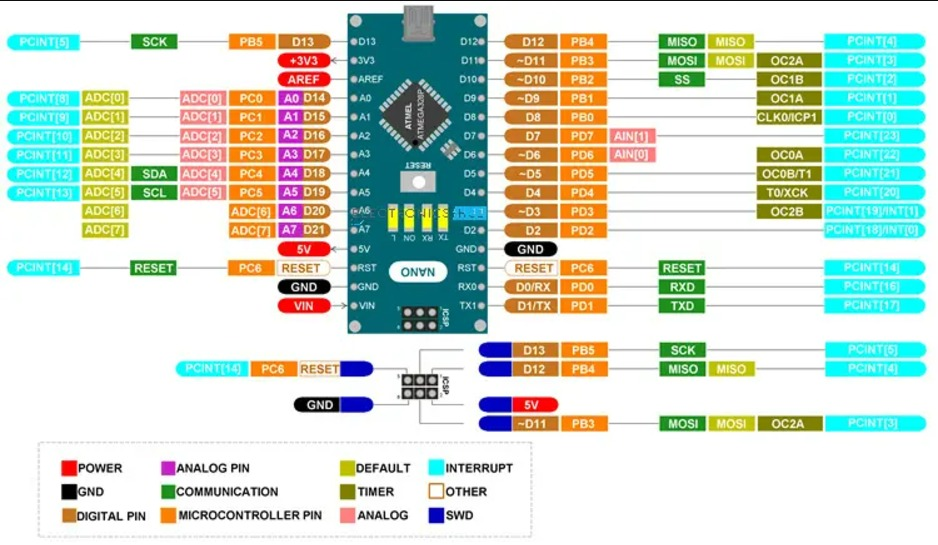
\includegraphics[scale=0.5]{WhatsApp Image 2024-12-02 at 1.06.30 PM.jpeg}
    \centering
    \caption{Arduino Nano connector Pin diagram}
    \label{fig:fig6}
\end{figure}




\pagebreak
\subsection{Results of Objective-III}
\textbf{Circuit Diagram of Hardware}
\begin{figure}[h!]
    \centering
    \begin{subfigure}
        \centering
        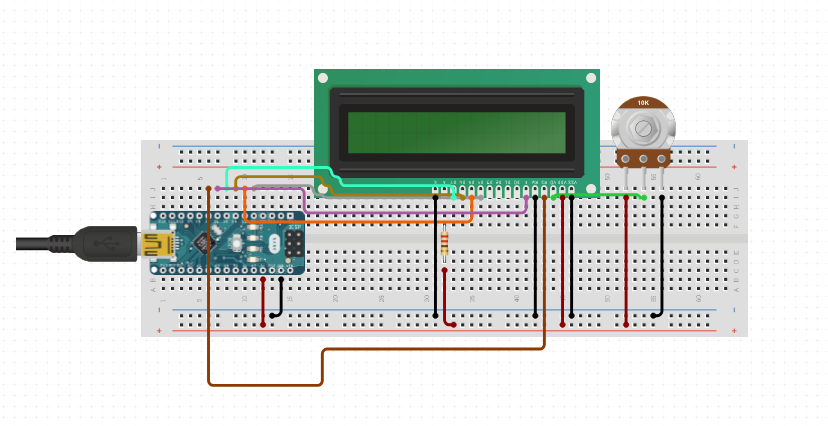
\includegraphics[width=\textwidth,keepaspectratio]{figures/circuit_rx.png}
        \caption{Circuit of Tx}
        \label{fig:Figure 5}
    \end{subfigure}
    \hfill
    \begin{subfigure}
        \centering
        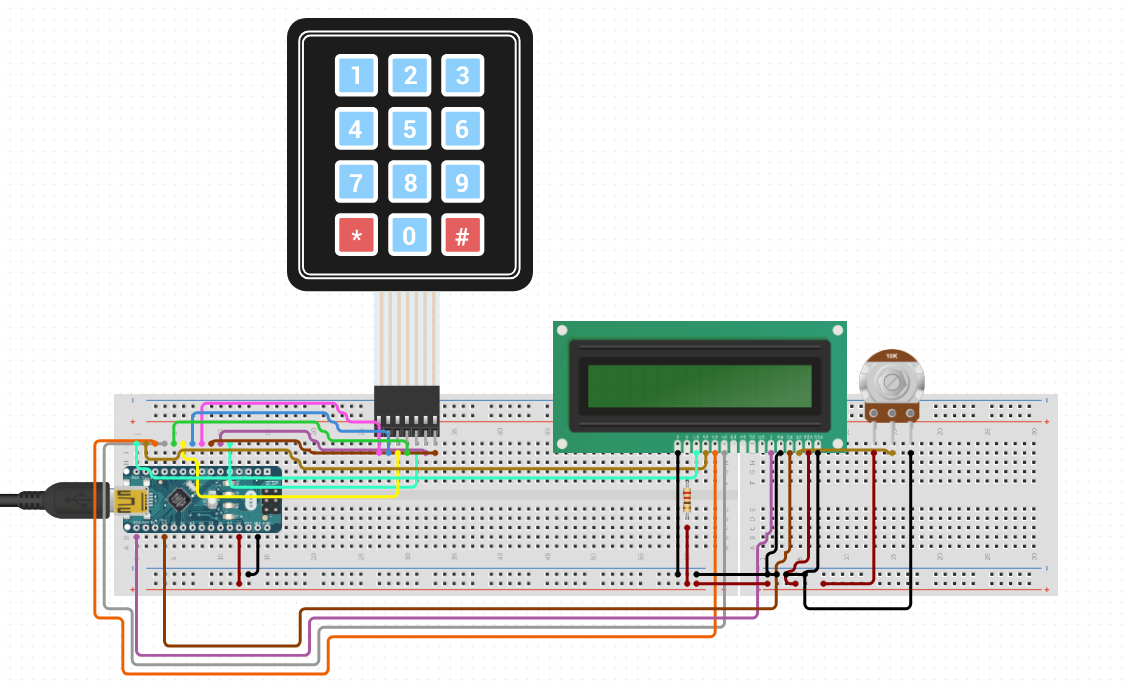
\includegraphics[width=\textwidth,keepaspectratio]{figures/circuit_tx.png}
        \caption{circuit of transmitter}
        \label{fig:Figure 6}
    \end{subfigure}
    % \caption{Overall caption for both images.}
    \label{fig:side_by_side_images}
\end{figure}


% \textbf{Circuit of Transmitter}
% \begin{figure}[htbp]
    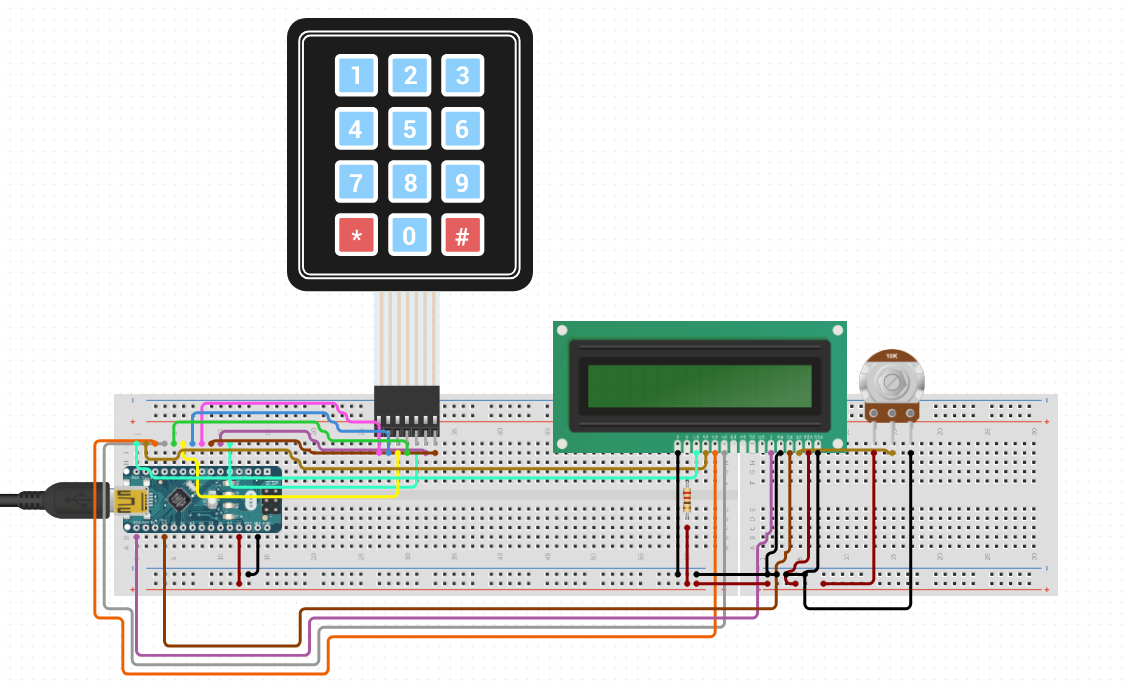
\includegraphics[width=7cm, keepaspectratio]{figures/circuit_tx.png}
    \centering
    \caption{circuit of Transmitter}
    \label{fig:fig7}
\end{figure}
% \textbf{Circuit of Reciever}
% \begin{figure}[htbp]
    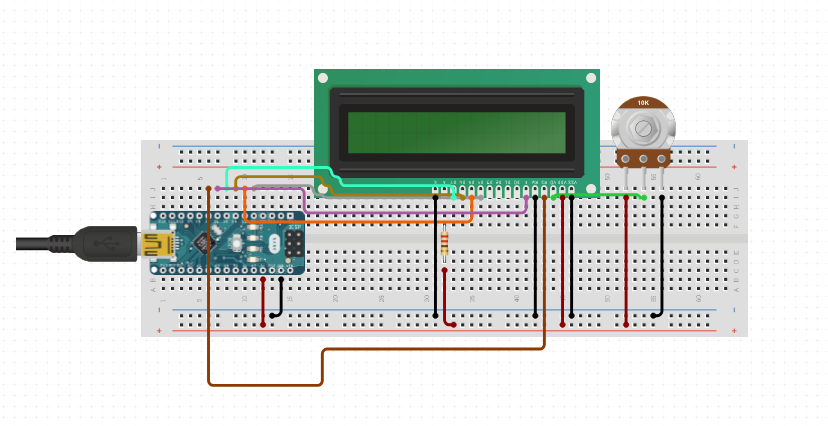
\includegraphics[width=7cm, keepaspectratio]{figures/circuit_rx.png}
    \centering
    \caption{circuit of Reciever}
    \label{fig:fig8}
\end{figure}

\textbf{Interfacing PS-2 keyboard with the Transmitter}
\begin{figure}[htbp]
    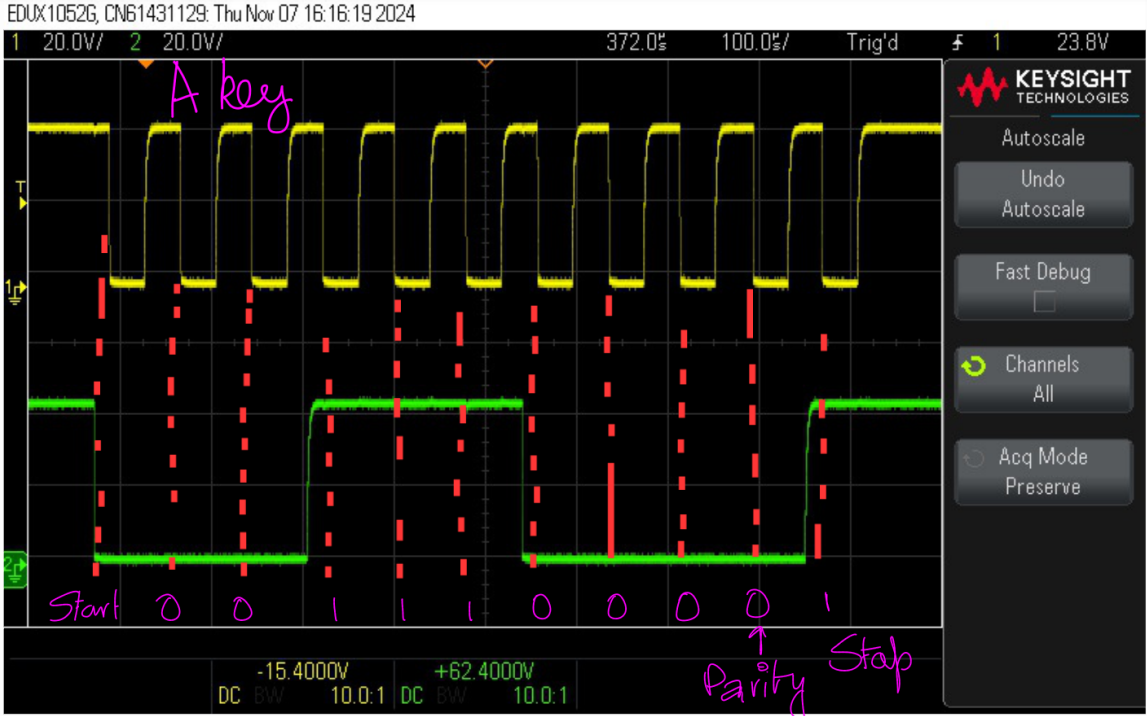
\includegraphics[width=14cm, keepaspectratio]{figures/ps2wav.png}
    \caption{PS-2 interface input wave}
    \label{fig:fig9}
\end{figure}
\textbf{Program to interpret the PS-2 Input}
% \pagebreak
\begin{figure}[htbp]
    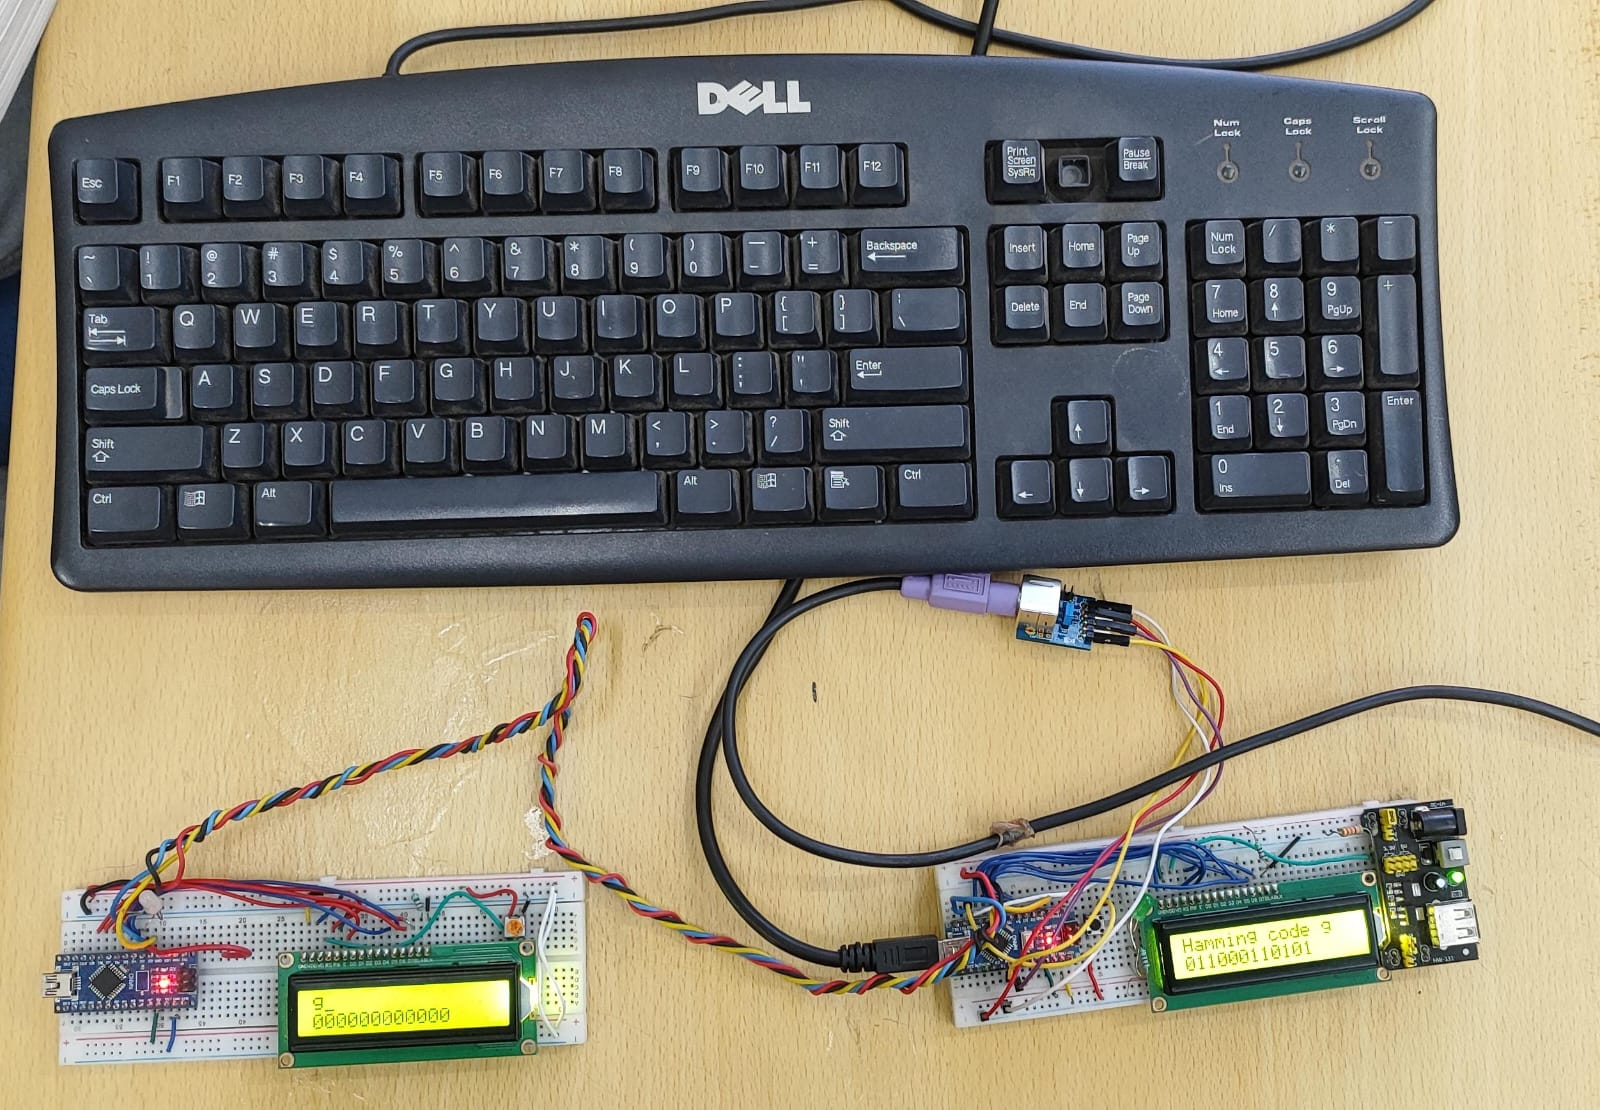
\includegraphics[width=14cm, keepaspectratio]{figures/propic.jpeg}
    \caption{Project image}
    \label{fig:fig5}
\end{figure}

\pagebreak
\subsection{Observation}
\begin{table}[h!]
        \centering
        \caption{Observation}\
        
        \
        \begin{tabular}{|c|c|}
            \hline
            \textbf{Character} & G \\
            \hline
            \textbf{Bit Type} & D8,D7,D6,D5,P8,D4,D3,D2,P4,D1,P2,P1 \\
            \hline
            \textbf{Binary} &  01000111 \\
            \hline
            \textbf{Hamming encoded} &  0100110111 \\
            \hline
            
        \end{tabular}
        
\end{table}
\begin{table}[h!]
        \centering
        \caption{Observation}\
       
        \
        \begin{tabular}{|c|c|}
            \hline
            \textbf{Character} & H \\
            \hline
            \textbf{Bit Type} & D8,D7,D6,D5,P8,D4,D3,D2,P4,D1,P2,P1 \\
            \hline
            \textbf{Binary} &  01001000 \\
            \hline
            \textbf{Hamming encoded} &  0100110111 \\
            \hline
            
        \end{tabular}
        
\end{table}
\begin{table}[h!]
        \centering
        \caption{Observation}\
       
        \
        \begin{tabular}{|c|c|}
            \hline
            \textbf{Character} & M \\
            \hline
            \textbf{Bit Type} & D8,D7,D6,D5,P8,D4,D3,D2,P4,D1,P2,P1 \\
            \hline
            \textbf{Binary} &  01001101 \\
            \hline
            \textbf{Hamming encoded} &  0100110111 \\
            \hline
            
        \end{tabular}
        
\end{table}
\begin{table}[h!]
        \centering
        \caption{Observation}\
        
        \
        \begin{tabular}{|c|c|}
            \hline
            \textbf{Character} & A \\
            \hline
            \textbf{Bit Type} & D8,D7,D6,D5,P8,D4,D3,D2,P4,D1,P2,P1 \\
            \hline
            \textbf{Binary} &  01000001 \\
            \hline
            \textbf{Hamming encoded} &  100010010001 \\
            \hline
            
        \end{tabular}
        
\end{table}

\begin{table}[h!]
        \centering
        \caption{Observation}\
       
        \
        \begin{tabular}{|c|c|}
            \hline
            \textbf{Character} & B \\
            \hline
            \textbf{Bit Type} & D8,D7,D6,D5,P8,D4,D3,D2,P4,D1,P2,P1 \\
            \hline
            \textbf{Binary} &   01000010 \\
            \hline
            \textbf{Hamming encoded} &  010110010010 \\
            \hline
            
        \end{tabular}
        
\end{table}


\begin{table}[h!]
        \centering
        \caption{Observation}\

        \
        \begin{tabular}{|c|c|}
            \hline
            \textbf{Character} & C \\
            \hline
            \textbf{Bit Type} & D8,D7,D6,D5,P8,D4,D3,D2,P4,D1,P2,P1 \\
            \hline
            \textbf{Binary} &  01000011 \\
            \hline
            \textbf{Hamming encoded} &  010010000011 \\
            \hline
            
        \end{tabular}
        
        
\end{table}

% \begin{table}[h!]
%         \centering
%         \caption{Observation}\

%         \
%         \begin{tabular}{|c|c|}
%             \hline
%             \textbf{Character} & D \\
%             \hline
%             \textbf{Bit Type} & D8,D7,D6,D5,P8,D4,D3,D2,P4,D1,P2,P1 \\
%             \hline
%             \textbf{Binary} &  01000100 \\
%             \hline
%             \textbf{Hamming encoded} &  110110010100 \\
%             \hline
            
%         \end{tabular}
        
% \end{table}

% \begin{table}[h!]
%         \centering
%         \caption{Observation}\
            
%             \
%         \begin{tabular}{|c|c|}
%             \hline
%             \textbf{Character} & E \\
%             \hline
%             \textbf{Bit Type} & D8,D7,D6,D5,P8,D4,D3,D2,P4,D1,P2,P1 \\
%             \hline
%             \textbf{Binary} &  01000101 \\
%             \hline
%             \textbf{Hamming encoded} &  110010000101 \\
%             \hline
            
%         \end{tabular}
        
% \end{table}

\pagebreak
\subsection{Test Scenarios}
Hamming code provides 1 bit Error Correction and 2 bits of Error Detection. The Test Scenarios are given below

\subsubsection{Single-bit Error Detection and Correction}
\textbf{Purpose:} Verify that the code detects and corrects single-bit errors. \\
\textbf{Test Case:} Inject a single-bit error at various positions in the encoded message. \\
\textbf{Example:} For a 7-bit Hamming Code (\texttt{0111000}), flip one bit (e.g., \texttt{1111000}) and check if the original message is recovered.

\subsubsection{Double-bit Error Detection}
\textbf{Purpose:} Ensure the code identifies that it cannot correct double-bit errors but can detect them. \\
\textbf{Test Case:} Flip two bits in the encoded message and observe the failure to decode accurately. \\
\textbf{Example:} Inject errors into positions 2 and 5 of \texttt{0111000}.

\subsubsection{Larger Message Sizes}
\textbf{Purpose:} Verify scalability of the implementation. \\
\textbf{Test Case:} Test with increasingly large input sizes (e.g., 16, 32, 64-bit messages). \\
\textbf{Example:} Use a 64-bit input and validate that encoding and error correction work correctly.

\subsubsection{No Errors}
\textbf{Purpose:} Ensure that no errors in transmission do not alter the message. \\
\textbf{Test Case:} Encode and decode a message without any injected errors. \\
\textbf{Example:} Input \texttt{1011} $\rightarrow$ Encode $\rightarrow$ Decode $\rightarrow$ Verify \texttt{1011}.

% ss

\subsubsection{Random Error Injection}
\textbf{Purpose:} Simulate real-world scenarios where errors occur randomly. \\
\textbf{Test Case:} Randomly flip bits in the encoded message across multiple runs. \\

\pagebreak
    
\section{\centering Conclusions and Scope for Future Works}
Key findings of Hamming code implementation include:
\begin{itemize}
    \item \textbf{Error Detection and Correction Capability:} Hamming codes detect and correct single-bit errors, which enhances communication system reliability.
    \item \textbf{Low Complexity:} The encoding and decoding processes are computationally lightweight, suitable for real-time applications.
    \item \textbf{Hardware Efficiency:} Hamming codes can be effectively implemented in both software and hardware, including FPGA and ASIC designs.
\end{itemize}

% \textbf{Practical Implications}

% The practical implications of implementing Hamming code are extensive. In modern systems, the ability to ensure data reliability is essential, and Hamming code provides a balance between complexity and error-correction capability. Key applications include:
% \begin{itemize}
 

% \item {Communication Systems}
% Hamming codes are commonly used in communication protocols to detect and correct errors in data packets. This reduces retransmission, leading to faster and more reliable data transfers.

% \item {Memory Systems}
% In computer memory systems such as RAM and cache memory, Hamming code is used for error correction to ensure data integrity during read and write operations. ECC (Error-Correcting Code) memory uses Hamming codes to automatically correct errors without user intervention.

% \item {Storage Devices}
% Hamming codes are implemented in storage devices like hard drives, SSDs, and data storage systems to maintain data integrity, especially in the presence of noise or wear-related errors.
% \end{itemize}

\textbf{Scope for Future Work}
While Hamming codes provide a strong foundation for error detection and correction, further enhancements can extend their capabilities for evolving applications. Future work can focus on the following aspects:
\begin{itemize}

\item {Hardware Optimization}

Optimizing the hardware implementation of Hamming code, including faster encoding and decoding circuits, can benefit real-time communication and memory systems. This involves reducing power consumption, increasing speed, and enhancing scalability.

\item {Integration with Modern Protocols}

As communication protocols continue to evolve, integrating Hamming codes into modern network and communication standards, including wireless networks, 5G systems, and IoT applications.

\item {Quantum Error Correction}

Exploring the application of Hamming code principles in quantum computing environments, where quantum error correction is essential, can open new research directions and lead to novel hybrid quantum-classical solutions.
\end{itemize}
In conclusion, Hamming code remains a fundamental approach for error detection and correction. Continued research and development can expand its applications, making it more relevant for emerging technologies and critical communication systems.

\pagebreak





 
  



    
\bibliographystyle{plain}
\bibliographystyle{IEEEtran}
\bibliography{references}

\end{document}
